%%%%%%%%%%%%%%%%%%%%%%%%%
% Dokumentinformationen %
%%%%%%%%%%%%%%%%%%%%%%%%%
\newcommand{\titleinfo}{Elektrische Maschinen - Formelsammlung}
\newcommand{\authorname}{\href{mailto:sreinli@hsr.ch}{S. Reinli} \quad \href{mailto:lmazzole@hsr.ch}{L. Mazzoleni}}
\newcommand{\authoremail}{\href{mailto:sreinli@hsr.ch}{sreinli@hsr.ch} \quad \href{mailto:lmazzole@hsr.ch}{lmazzole@hsr.ch} }
\newcommand{\versioninfo}{$ Revision: 1.1 $}

%NEWCOMMANDS überarbeiten
%wieso mit new Command? Author Email Info besser aufteilen

%%%%%%%%%%%%%%%%%%%%%%%%%%%%%%%%%%%%%%%%%%%%%
% Standard projektübergreifender Header für 
% - Makros 
% - Farben
% - Mathematische Operatoren
%
% dORT NUR ERGÄNZEN, NICHTS LÖSCHEN
%%%%%%%%%%%%%%%%%%%%%%%%%%%%%%%%%%%%%%%%%%%%%
% Genereller Header
\documentclass[11pt,twoside,a4paper,fleqn]{article}
% Dateiencoding
\usepackage[utf8]{inputenc}
\usepackage[T1]{fontenc}	%ä,ü...
% Seitenränder
\usepackage[left=1cm,right=1cm,top=1cm,bottom=1cm,includeheadfoot]{geometry}
% Sprachpaket
\usepackage[english, ngerman]{babel} % Silbentrennung und Rechtschreibung Englisch und Deutsch

%%%%%%%%%%%%%%%%%%%%%%%
%% Wichtige Packages %%
%%%%%%%%%%%%%%%%%%%%%%%
\usepackage{amssymb,amsmath,fancybox,graphicx,color,lastpage,wrapfig,fancyhdr,hyperref,verbatim,floatflt,multicol,multirow,rotating,pdflscape,array,longtable,listings,trfsigns,trsym,tabularx,mathtools,mathabx}

% Zum Bilder einfach in Tabellen einfügen (valign=t)
\usepackage[export]{adjustbox}

% Für Abbildungen mit mehreren kleinen Bilder
% Doku: http://www.ctan.org/tex-archive/macros/latex/contrib/caption/
\usepackage{caption}
\usepackage{subcaption}


%%%%%%%%%%%%%%%%%%%%
% Generelle Makros %
%%%%%%%%%%%%%%%%%%%%
\newcommand{\skript}[1]{$_{\textcolor{red}{\mbox{\small{Skript S.#1}}}}$}
\newcommand{\verweis}[2]{\small{(siehe auch \ref{#1}, #2 (S. \pageref{#1}))}}
\newcommand{\verweiskurz}[1]{(\small{siehe \ref{#1}\normalsize)}}
\newcommand{\subsubadd}[1]{\textcolor{black}{\mbox{#1}}}
\newcommand{\formelbuch}[1]{$_{\textcolor{red}{\mbox{\small{S#1}}}}$}

\newcommand{\kuchling}[1]{$_{\textcolor{red}{\mbox{\small{Kuchling #1}}}}$}
\newcommand{\stoecker}[1]{$_{\textcolor{grey}{\mbox{\small{Stöcker #1}}}}$}
\newcommand{\sachs}[1]{$_{\textcolor{blue}{\mbox{\small{Sachs S. #1}}}}$}
\newcommand{\hartl}[1]{$_{\textcolor{green}{\mbox{\small{Hartl S. #1}}}}$}

\newcommand{\schaum}[1]{\tiny Schaum S. #1}

\newcommand{\skriptsection}[2]{\section{#1 {\tiny Skript S. #2}}}
\newcommand{\skriptsubsection}[2]{\subsection{#1 {\tiny Skript S. #2}}}
\newcommand{\skriptsubsubsection}[2]{\subsubsection{#1 {\tiny Skript S. #2}}}

\newcommand{\matlab}[1]{\footnotesize{(Matlab: \texttt{#1})}\normalsize{}}

% Syntax: \bmu{Pfad zum Bild}{Bildgrösse}{Beschriftung des Bildes}
\newcommand{\bl}[2]{
	\begin{figure}[h]
		\flushleft  % linksbuendig
		\includegraphics[width=#1]{#2} \\
	\end{figure}
}
\newcommand{\br}[2]{
	\begin{figure}[h]
		\flushright  % rechtsbuendig
		\includegraphics[width=#1]{#2} \\
	\end{figure}
}

\newcommand{\bild}[2]{
	\begin{figure}[h]
		\centering  % zentriert
		\includegraphics[width=#1]{#2} \\
	\end{figure}
}

\newcommand\tabbild[2][]{%
	\raisebox{0pt}[\dimexpr\totalheight+\dp\strutbox\relax][\dp\strutbox]{%
		\includegraphics[#1]{#2}%
	}%
}
\newcolumntype{P}[1]{>{\raggedright\arraybackslash}p{#1}} %Tabelle linksausgerichtet
\newcolumntype{L}[1]{>{\raggedleft\arraybackslash}p{#1}} %Tabelle rechtsausgerichtet
\newcolumntype{C}[1]{>{\centering\arraybackslash}p{#1}}
\definecolor{mygray}{RGB}{190, 190, 190}
\def\Int{\mbox{\Large$\displaystyle\int$\normalsize}}
\def\OInt{\mbox{\Large$\displaystyle\oint$\normalsize}}



%%%%%%%%%%
% Farben %
%%%%%%%%%%
\definecolor{black}{rgb}{0,0,0}
\definecolor{red}{rgb}{1,0,0}
\definecolor{white}{rgb}{1,1,1}
\definecolor{grey}{rgb}{0.8,0.8,0.8}
\definecolor{green}{rgb}{0,.8,0.05}
\definecolor{brown}{rgb}{0.603,0,0}


%%%%%%%%%%%%%%%%%%%%%%%%%%%%
% Mathematische Operatoren %
%%%%%%%%%%%%%%%%%%%%%%%%%%%%
\DeclareMathOperator{\sinc}{sinc}
\DeclareMathOperator{\sgn}{sgn}
\DeclareMathOperator{\Real}{Re}
\DeclareMathOperator{\Imag}{Im}
%\DeclareMathOperator{\e}{e}
\DeclareMathOperator{\cov}{cov}
\DeclareMathOperator{\PolyGrad}{PolyGrad}

%Makro für 'd' von Integral- und Differentialgleichungen 
\newcommand*{\diff}{\mathop{}\!\mathrm{d}}


%%%%%%%%%%%%%%%%%%%%%%%%%%%
% Fouriertransformationen %
%%%%%%%%%%%%%%%%%%%%%%%%%%%

% Fouriertransformationen
\unitlength1cm
\newcommand{\FT}
{
	\begin{picture}(1,0.5)
	\put(0.2,0.1){\circle{0.14}}\put(0.27,0.1){\line(1,0){0.5}}\put(0.77,0.1){\circle*{0.14}}
	\end{picture}
}


\newcommand{\IFT}
{
	\begin{picture}(1,0.5)
	\put(0.2,0.1){\circle*{0.14}}\put(0.27,0.1){\line(1,0){0.45}}\put(0.77,0.1){\circle{0.14}}
	\end{picture}
}

%%%%%%%%%%%%%%%%%%%%%%%%%%%%
% Allgemeine Einstellungen %
%%%%%%%%%%%%%%%%%%%%%%%%%%%%
%PDF Info
\hypersetup{pdfauthor={\authorinfo},pdftitle={\titleinfo},colorlinks=false}
\author{\authorinfo}
\title{\titleinfo}

%%%%%%%%%%%%%%%%%%%%%%%
% Kopf- und Fusszeile %
%%%%%%%%%%%%%%%%%%%%%%%
\pagestyle{fancy}
\fancyhf{}
%Linien oben und unten
\renewcommand{\headrulewidth}{0.5pt} 
\renewcommand{\footrulewidth}{0.5pt}

\fancyhead[L]{\titleinfo{ }\tiny{(\versioninfo)}}
%Kopfzeile rechts bzw. aussen
\fancyhead[R]{Seite \thepage { }von \pageref{LastPage}}
%Fusszeile links bzw. innen
\fancyfoot[L]{\footnotesize{\authorinfo}}
%Fusszeile rechts bzw. ausen
\fancyfoot[R]{\footnotesize{\today}}
% Einrücken verhindern versuchen
\setlength{\parindent}{0pt}

% Zeilenhöhe Tabellen:
\newcommand{\arraystretchOriginal}{1.5}
\renewcommand{\arraystretch}{\arraystretchOriginal}




%\usepackage{circuitikz}
% Möglichst keine Ergänzungen hier, sondern in header.tex

%%%%%%%%%%%%%%%%%%%%%%%%%%%%%%%%%%%%%%%%%%%%%%%%%%%%%%%%%%%%%%%%%%%%%%%%%%%%%%%%%%%%%%%%%%%%%%%%
%%%%%%%%%%%%%%%%%%%%%%%%%%%%%%%%%%%%%%%%%%%%%%%%%%%%%%%%%%%%%%%%%%%%%%%%%%%%%%%%%%%%%%%%%%%%%%%%

\begin{document}
\maketitle
\vspace{-2.5cm}
\setcounter{tocdepth}{2}
\tableofcontents
\thispagestyle{empty}
\pagebreak
\section{Grundlagen}
\subsection{Wichtige Formeln}
    \begin{longtable}{| p{.25\textwidth} | p{.40\textwidth} | p{.30\textwidth} |}
        \firsthline
        \textbf{Elektrische Kraft} \newline
        \tabbild[width=3.5cm]{images/ElKraft.png}  &
        \begin{equation*}\vec{F_e} = \dfrac{1}{2\pi\epsilon}\cdot\dfrac{Q\cdot q}{r}\cdot\vec{r_0}\end{equation*}
        \begin{equation*}F_e = \dfrac{\pi\cdot U^2}{2\cdot r\cdot(\ln{\dfrac{r-R_1}{R_1}})^2}\end{equation*} & \newline
        [${F_e}$] = $\dfrac{N}{m}$\newline \newline 
        $\epsilon\;\widehat{=}\;$elektrische Permittivität\newline 
        $\epsilon_0 = 8.8542 \cdot 10^{-12}$ $\left[\dfrac{As}{Vm}\right]$ \newline \newline
        Q,q$\,\widehat{=}\,$Linienladungsdichten $\,\left[\dfrac{C}{m}\right]$ 
        \\ \hline
        
        \textbf{Magnetische Kraft} \newline
        \tabbild[width=3.5cm]{images/magnetischeKraft.png}  &	
        \begin{equation*}\vec{F_m} = \dfrac{\mu}{2\pi}\cdot\dfrac{I\cdot i}{r}\cdot\vec{r_0}\end{equation*} 
        \begin{equation*}F_m = \dfrac{\mu_0\cdot I^2}{2\cdot\pi\cdot r}\end{equation*} 
        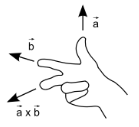
\includegraphics[width=3cm]{images/vektorprodukt.png}	& \newline
        $\mu$ $\widehat{=}$ magnetische Permeabilität\newline 
        $\mu_0$ = $4\pi\cdot 10^{-7} \,\left[\dfrac{N}{A^2}\right]=\left[\dfrac{Vs}{Am}\right]$ \newline \newline
        $\vec{r_0}=\dfrac{\vec{r}}{|\vec{r}|}$ \newline \newline 
        I, i $\widehat{=}$ elektrische Ströme 	\newline \newline 
        $[F_m]$ = $\dfrac{N}{m}$
        \\ \hline
        
        \textbf{Elektrisches Feld} \newline \newline
        \tabbild[width=4cm]{images/elektrischesFeld.png} &
        \begin{equation*}\vec{E} = \dfrac{\vec{F_e}}{q} = \dfrac{1}{2\pi\epsilon}\cdot\dfrac{Q}{r}\cdot\vec{r_0}\end{equation*} 
        \begin{equation*}\vec{E} = \dfrac{1}{2\pi\epsilon}\cdot\dfrac{Q}{r}\cdot\vec{r_0}\end{equation*} & 
        \begin{equation*}[E] = \dfrac{V}{m}\end{equation*} 									
        \\ \hline
        
        \textbf{Elektrisches Potential}  &
        \begin{equation*}\varphi = \int\vec{E}\cdot\vec{dl}	\end{equation*}	& 
        \begin{equation*}[\varphi] = V\end{equation*} 
        \\ \hline
        
        \textbf{Elektrische Spannung}   &
        \begin{equation*}U_{AB} = \int\limits_{A}^{B}\vec{E}\cdot\vec{dl} = \varphi_A - \varphi_B\end{equation*}  & 
        \begin{equation*}[U] = V \end{equation*}  
        \\ \hline
              
        \textbf{Elektrischer Strom} 	    &  
        \begin{equation*}I = \dfrac{dQ}{dt}	\end{equation*} &  
        \begin{equation*}[I] = A\end{equation*} 
        \\ \hline
        		
        \textbf{Magnetische Feldstärke} \newline \newline
        \tabbild[width=4cm]{images/magnetischesFeld.png} &
        \begin{equation*}\vec{H} = \dfrac{I}{2\pi}\cdot\dfrac{\vec{L_0}\times\vec{r_0}}{r} \end{equation*} & 
        \newline [H] = $\dfrac{A}{m}$ \newline
        $\vec{L_0},\vec{l_0}$ $\widehat{=}$ Einheitsvektoren der Stromleiter
        \\ \hline
        
        \textbf{Magnetische Flussdichte}  &
        \begin{equation*}\vec{B} = \mu\cdot\vec{H} = \mu_0\cdot\mu_r\cdot\vec{H}\end{equation*} &  
        \begin{equation*}[B] = T=\dfrac{Vs}{m^2}\end{equation*} 
        \\ \hline
        
        \textbf{Magnetische Fluss} \newline
        \tabbild[width=3.5cm]{images/magnetischeFluss} & 
        \begin{equation*}\phi = \iint\limits_{(A)}\vec{B}\cdot\vec{dA}\end{equation*} &  
        \begin{equation*}[\phi] = Vs = Wb\end{equation*}
        \\ \hline
        
        \textbf{Verkettete Fluss}\newline 
        \tabbild[width=5cm]{images/Verkettetefluss}		 &
        \begin{equation*}\psi = N\cdot\phi\end{equation*}
        \begin{equation*}\psi = L\cdot I\end{equation*}
        \centering\textbf{meistens} 
        \begin{equation*}\psi(t) = N\cdot\iint\limits_{(A)}\vec{B}\cdot\vec{dA}=N\cdot B \cdot A \cdot cos\left(\omega t\right)\end{equation*} & 
        \begin{equation*}[\psi] = Vs = Wb\end{equation*}
        \\ \hline
        
        \textbf{Induzierte Spannung} 	 &
        \begin{equation*}U_{ind} = -\dfrac{d\psi}{dt}=-N\dfrac{d\phi}{dt}\end{equation*}			
        \centering\textbf{meistens} 
        \begin{equation*}U_{ind} = -\dfrac{d\psi}{dt}=\omega\cdot N\cdot B\cdot A\cdot sin\left(\omega t\right)\end{equation*}  &
        \\ \hline
        
        \textbf{Magnetische Durchflutung} \newline \newline
        \tabbild[width=5cm]{images/Durchflutungssatz.png}  &
        \begin{equation*}	 \Theta = \sum\limits_{k=1}^{n}I_k = \oint\limits_{(C)}\vec{H}\cdot\vec{dl}\end{equation*}  
        \centering\textbf{Beispiel:}\
        \begin{equation*}	\oint\limits_{(C)}\vec{H}\cdot\vec{dl} = \int \limits_{P_1}^{P_2}\vec{H}\cdot\vec{dl} + \int \limits_{P_2}^{P_3}\vec{H}\cdot\vec{dl}	+ ... + \int \limits_{P_{m-1}}^{P_m}\vec{H}\cdot\vec{dl}\end{equation*}				&
        \begin{equation*}[\Theta] = A\end{equation*} 
        \\ \hline
        
        \textbf{Magnetische Spannung}	 & 
        \begin{equation*}V_m = \int\limits_{A}^{B}\vec{H}\cdot\vec{dl}\end{equation*}											
        & \begin{equation*}[V_m] = A\end{equation*} 
        \\ \hline 
        
        \textbf{Magnetkreis}	\newline
        \tabbild[width=5cm]{images/magnetkreis.png}  &
        \begin{equation*}\oint\limits_{(C)}\vec{H}\cdot\vec{dl} \approx H\cdot L = N\cdot I\end{equation*}  
        \begin{equation*}\Rightarrow H = \dfrac{N\cdot I}{L}\end{equation*} 
        \begin{equation*}\Rightarrow B = \mu_0\cdot\dfrac{N\cdot I}{L}\end{equation*} &    
        falls L $>>$ R und \newline 
        das Feld in der Spule \textbf{homogen} ist
        \\ \hline
        
        \textbf{Reluktanzkraft} \newline
        \tabbild[width=4cm]{images/reluktanzkraft.png} &
        \begin{equation*}F_R = -\dfrac{\partial W_m}{\partial\delta} = \mu_0\cdot\dfrac{N^2\cdot I^2\cdot A_{Fe}}{4\cdot\delta^2}\end{equation*} & 
        wobei $A_{Fe}$ die magnetisch wirksame Fläche des Luftspalts ist. 
        \\ \hline
        
        \textbf{magnetische Energie} & \begin{equation*}
        W_m = \dfrac{1}{2}\cdot H_\delta\cdot B_\delta\cdot2\cdot A_{Fe}\cdot\delta = \mu_0\cdot \dfrac{I^2\cdot N^2}{4\cdot\delta}\cdot A_{Fe}
        \end{equation*} & wobei $A_{Fe}\cdot\delta$ dem Volumen des Luftspalts entspricht. \\
        \lasthline
    \end{longtable}
    \clearpage
    \newpage

\subsection{Elektrische Kraft vs. Magnetische Kraft}
    \begin{minipage}{0.5\textwidth}
    	\centering
        \textcolor{red}{\begin{equation*}F_e\, = \dfrac{\pi\cdot\epsilon_0\cdot U^2}{2\cdot r\cdot\left(ln\dfrac{r-R_1}{R_1}\right)^2} = 2.88\cdot 10^{-11} \quad \left[\dfrac{N}{m}\right]\end{equation*}}
        \end{minipage}
        \begin{minipage}{0.5\textwidth}
        	\centering
        \textcolor{blue}{\begin{equation*}F_m = \dfrac{\mu_0\cdot I^2}{2\cdot\pi\cdot r} = 2.00 \cdot 10^{-6} \quad\left[\dfrac{N}{m}\right]\end{equation*}}
    \end{minipage}
    \begin{enumerate}
    	\item Der Absolutbetrag der magnetischen Kraft pro Längen- und Stromeinheit ist
    	ungefähr $7\cdot10^4$ mal grösser als der entsprechende Betrag der elektrischen Kraft
    	pro Längen- und Spannungseinheit.
    	\item Um die Kraft von 1 (N/m) in dieser Anordnung zu erzeugen ist entweder der
    	Strom von ungefähr 700A oder die Spannung von ungefähr 600’000V notwendig.
    	\item \textcolor{red}{\textbf{Die Argumenten 1 und 2 deuten daraufhin, dass die magnetische Kraft für die Energieumwandlung besser als die elektrische Kraft geeignet ist.}}\\[0.2cm]
    	Deswegen basieren die modernen elektrischen Maschinen hauptsächlich auf der magnetischen Kraft.
    \end{enumerate}
\clearpage
\newpage
\section{GSM - Gleichstrommotoren}
    
    \vspace{-0.5cm}
    \begin{minipage}[b]{0.45\textwidth}
    	\centering
    	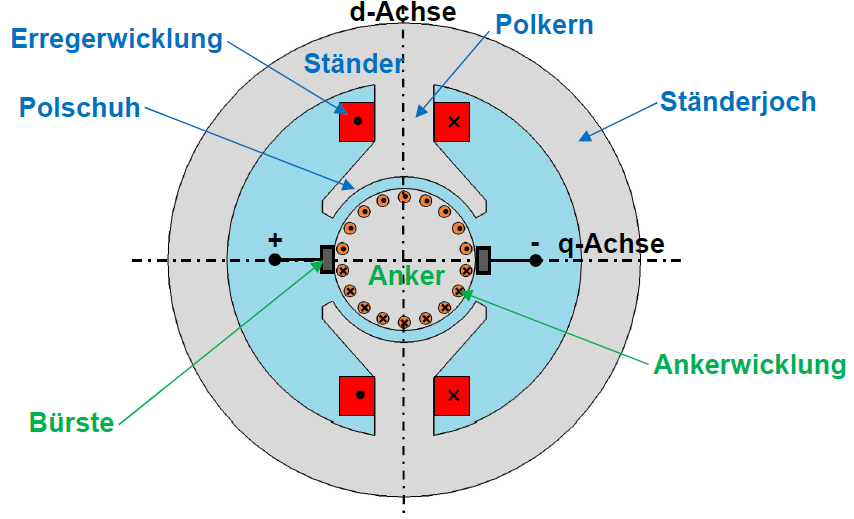
\includegraphics[width=8cm]{images/GSM_Aufbau.png}
    \end{minipage}
    \begin{minipage}[b]{0.25\textwidth}
    	\centering
    	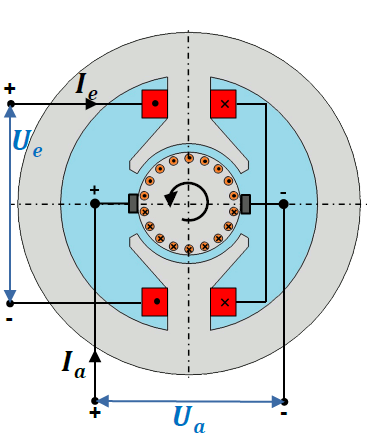
\includegraphics[width=5cm]{images/Grundgleichungen.png}
    	\vspace{-1cm}
    \end{minipage}
    \begin{minipage}[b]{0.33\textwidth}
    	\vspace{-2cm}
    	\centering
    	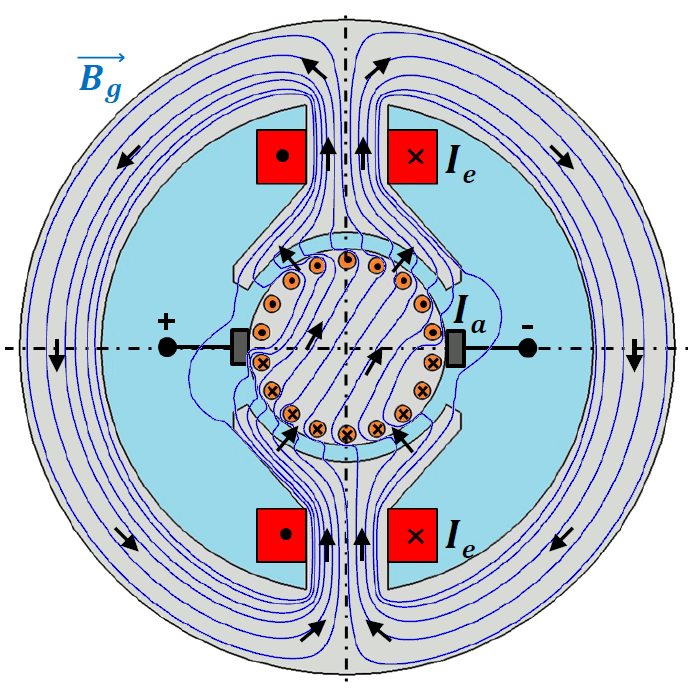
\includegraphics[width=5cm]{images/Ankerrueckwirkung.png}
    	\vspace{0.2cm}
    \end{minipage}
    \vspace{-1cm}
    
    \subsection{Fremderregte GSM}
    \vspace{-0.2cm}
    \begin{minipage}[b]{0.5\textwidth}
    	\raggedright
    	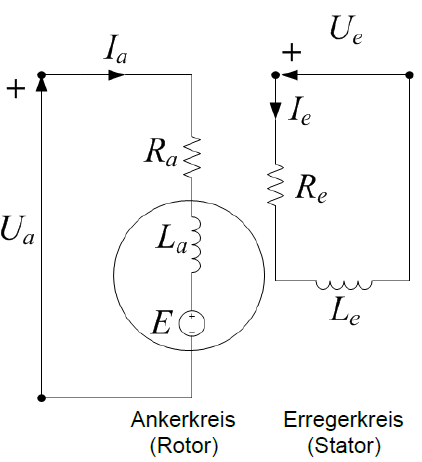
\includegraphics[width=6cm]{images/Ersatzschaltbild_GSM.png}
    \end{minipage}
    \begin{minipage}[b]{0.5\textwidth}
    	\raggedright
    	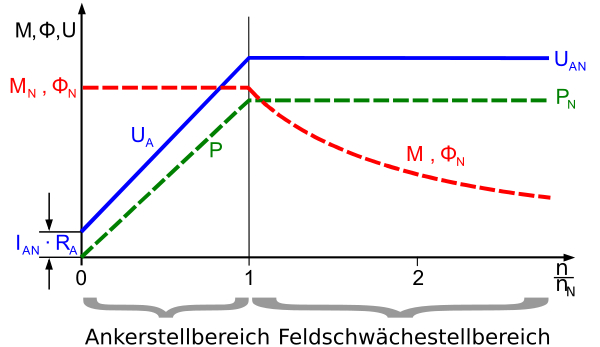
\includegraphics[scale = 0.7]{images/KennlinieFremderregt}
    \end{minipage}\\
    
    \begin{longtable}{| p{.25\textwidth} | p{.40\textwidth} | p{.30\textwidth} |}
        \firsthline
        \textbf{Erregerwicklung}	&
        $U_e = R_e\cdot I_e + L_e\cdot\dfrac{dI_e}{dt}$ &
        Spannungsgleichung des Statorkreises
        \\ \hline
        
        \textbf{Ankerwicklung}	&
        \[ U_a = R_a \cdot I_a + L_a \cdot \dfrac{dI_a}{dt} + E \] &
        $E = \omega\cdot\psi$
        \qquad $\psi = L_e\cdot I_e \, \widehat{=}$ Erregerfluss \newline \newline
        $\omega = 2\pi\cdot n$ \newline
        \quad n $\widehat{=}$ Drehzahl des Läufers $\left[\dfrac{1}{s}\right]$\newline \newline Spannungsgleichung des Rotorkreises
        \\ \hline
        
        \textbf{Elektrische Leistung} &
        Im stationären Betrieb: \quad $\left(\dfrac{d}{dt} = 0\right)$ \newline \newline
        $P_{el} = P_e + P_a = U_e\cdot I_e + U_a\cdot I_a$ \newline \newline
        $P_{el} = \underbrace{R_e\cdot I_e^2}_{\substack{Ohmsche \\ Erregerverluste}} + \underbrace{R_a\cdot I_a^2}_{\substack{Ohmsche \\ Ankerverluste}} + \underbrace{\omega\cdot\psi\cdot I_a}_{\substack{Mechanische\\Leistung}}$ \newline &
        $[P] = W$
        \\ \hline
        
        \textbf{Mechanische Leistung} &
        $P_{mech} = \omega\cdot M = \omega\cdot\psi\cdot I_a\, = \omega\cdot L_e \cdot I_e \cdot I_a$ &
        \\ \hline
        
        \textbf{Drehmoment} &
        $M = \psi\cdot I_a\, = L_e\cdot I_e\cdot I_a$ &
        $[M] = Nm$
        \\ \lasthline
    \end{longtable}
    \clearpage
    \newpage

\subsection{Nebenschluss GSM}
    Die Erreger- und Ankerwicklung werden parallel an die gleiche Spannungsquelle geschaltet.\newline Beim Nebenschluss sind die Anker- und Erregerspannung gleich und der Anker- und Erregerstrom unabhängig \newline voneinander. \\
    \begin{minipage}[b]{0.4\textwidth}
    	\raggedright
    	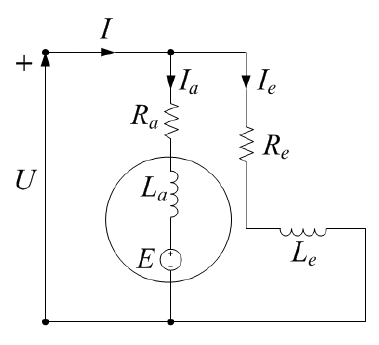
\includegraphics[width=6cm]{images/Nebenschluss_GSM.png}
    \end{minipage}
    \begin{minipage}[b]{0.5\textwidth}
    	\raggedright
    	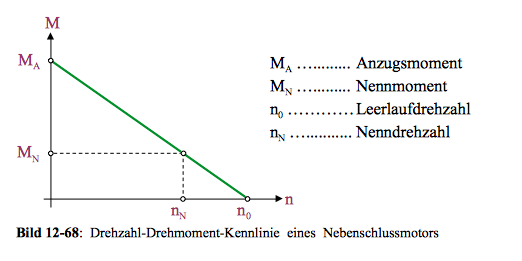
\includegraphics[scale = 0.6]{images/KennlinieNebenschluss}
    \end{minipage}\\
    
    %\renewcommand{\arraystretch}{2.5}
    \begin{longtable}{| p{.25\textwidth} | p{.40\textwidth} | p{.30\textwidth} |}
    	\firsthline
    	\textbf{Drehmoment}	&
        $U = U_a = R_a\cdot I_a + \omega\cdot\psi$ \newline \newline
        $I_a = \dfrac{U - \omega\cdot\psi}{R_a}$ \newline \newline
        $M = I_a\cdot\psi\, = \, I_a \cdot L_e \cdot I_e $ \newline\newline
        $M = \dfrac{U\cdot\psi}{R_a}-\dfrac{\omega\cdot\psi^2}{R_a}$ \newline &
        Spannungsgleichung der Nebenschluss-Schaltung\newline \newline
        $\psi = L_e\cdot I_e \, \widehat{=}$ Erregerfluss \newline \newline
        $\omega\, = \, 2\pi\cdot n \quad \left[\dfrac{1}{s}\right]$
        \\ 	\hline
        
    	\textbf{Anlaufmoment} \newline \newline
        $(n = 0)$	&
        $M_A = \dfrac{U\cdot\psi}{R_a + R_v}$ \newline \newline
        $I_{Anlauf} \,= \, \dfrac{U}{R_a + R_v} $ &
        $[M] = Nm$ \newline
        $R_a \, \widehat{=}$\, Ankerwiderstand \newline
        $R_v \, \widehat{=}$ Im Ankerkreis in Serie geschalteter Regelungswiderstand (= \textbf{oft 0})
        \\ \hline
        
    	\textbf{Elektrische Leistung} &
        Im stationären Betrieb: \quad $\left(\dfrac{d}{dt} = 0\right)$ \newline \newline
        $P_{el} = P_e + P_a = U_e\cdot I_e + U_a\cdot I_a$ \newline \newline
        $P_{el} = \underbrace{R_e\cdot I_e^2}_{\substack{Ohmsche \\ Erregerverluste}} + \underbrace{R_a\cdot I_a^2}_{\substack{Ohmsche \\ Ankerverluste}} + \underbrace{\omega\cdot\psi\cdot I_a}_{\substack{Mechanische\\Leistung}}$ \newline &
        $[P] = W$
        \\ \hline
        
    	\textbf{Mechanische Leistung} &
        $P_{mech} = \omega\cdot M = \omega\cdot\psi\cdot I_a$ &
        \\ \hline
        
    	\textbf{Leerlaufdrehzahl}&
        $n_0 = \dfrac{U}{2\pi\cdot\psi}$  \qquad $(M = 0)$&
        $[n] = \dfrac{1}{s}$
        \\ \lasthline
    \end{longtable}
    \clearpage
    \newpage

\subsection{Reihenschluss GSM}
    Die Erreger- und Ankerwicklung werden in Serie an die gemeinsame Spannungsquelle geschaltet.\newline Beim Reihenschluss sind die Anker- und Erregerströme gleich und die Anker- und Erregerspannungen sind deshalb \newline stark voneinander abhängig.\newline
    \begin{minipage}[b]{0.4\textwidth}
    	\raggedright
    	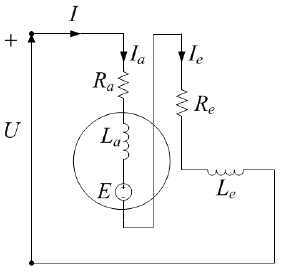
\includegraphics[width=6cm]{images/Reihenschluss.png}
    \end{minipage}
    \begin{minipage}[b]{0.5\textwidth}
    	\raggedright
    	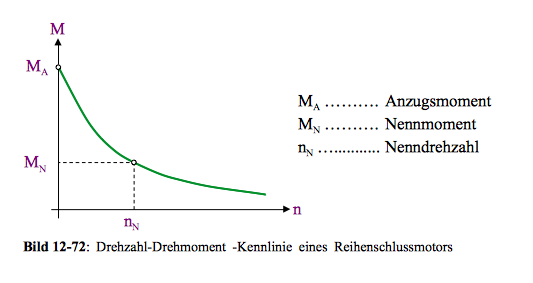
\includegraphics[scale = 0.6]{images/KennlinieReihenschluss}
    \end{minipage}\\
    \begin{minipage}[b]{0.7\linewidth}
        \raggedleft
        \textcolor{red}{Achtung: M $\rightarrow$ 0 $\Rightarrow$ n $\rightarrow \infty$}
    \end{minipage}
    \\
    
    \begin{longtable}{| p{.25\textwidth} | p{.40\textwidth} | p{.30\textwidth} |}
    	\firsthline
    	\textbf{Drehmoment}	&
        $U = (R_a + R_e)\cdot I + 2\pi n\cdot\psi$ \newline \newline
        $M = I\cdot\psi$ \newline \newline
        $M = I\cdot\psi = L_e\cdot\left(\dfrac{U}{R_a + R_e + 2\pi n\cdot\psi}\right)^2$\newline\newline
        $\psi = L_e\cdot I$ & Spannungsgleichung der Reihenschluss-Schaltung \newline \newline $I\,=\,I_a\,=\,I_e$
        \\\hline
        
    	\textbf{Anlaufmoment}	&
        $M_A = \dfrac{L_e\cdot U^2}{\left(R_a + R_e\right)^2}$ \qquad $\left(n = 0\right)$ &
        $[M] = Nm$ 
        \\ \hline
        
    	\textbf{Bezugsdrehzahl}&
        $n_b = \dfrac{R_a + R_e}{2\pi\cdot L_e}$ \newline &
        $[n] = \dfrac{1}{s}$
        \\ \lasthline
    \end{longtable}

\subsection{Drehzahlregelung}
    \begin{minipage}[b]{0.33\textwidth}
    	\raggedright
    	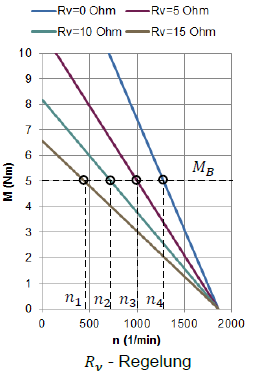
\includegraphics[width=5cm]{images/Widerstandsregelung.png}
    \end{minipage}
    \begin{minipage}[b]{0.33\textwidth}
    	\raggedright
    	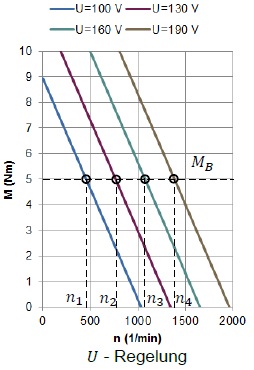
\includegraphics[width=5cm]{images/Spannungsregelung.png}
    \end{minipage}
    \begin{minipage}[b]{0.33\textwidth}
    	\raggedright
    	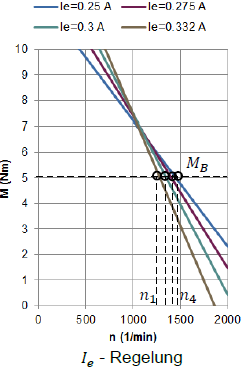
\includegraphics[width=5cm]{images/Erregerstromregelung.png}
    \end{minipage}
    \clearpage
    \newpage







\section{Dreiphasenwechselstrom und Drehfelderzeugung}
    \begin{tabular}[b]{| C{4cm} | P{5cm} | P{9cm} |}
    	\hline
        \textbf{Sternspannungen} &
        $U_U(t) = U_m\cdot\sin\left(\omega t\right)$ \newline \newline
        $U_V(t) = U_m\cdot\sin\left(\omega t - \dfrac{2\pi}{3}\right)$ \newline \newline
        $U_W(t) = U_m\cdot\sin\left(\omega t - \dfrac{4\pi}{3}\right)$ &
        $U_U, U_V, U_W \,\widehat{=}$ den Spannungen zwischen dem Neutralleiter und dem Aussenleiter
        \\ \hline
        
        \textbf{Stern-Dreieck Umwandlung}&
        $ U_Y= \frac{U_\Delta}{3} $\newline
        $ I_Y= \frac{I_\Delta}{3} $ \newline
        $ M_Y= \frac{M_\Delta}{3} $&
        $U = Strangspannung [V] $\newline
        $I = Strangstrom [A] $\newline
        $M = Motormoment [Nm] $
        \\ \hline
                
        \textbf{Verkettete Spannung} & 	&
        $U_{UV}, U_{VW}, U_{WU}$
        \\ \hline
    \end{tabular}
    \\[0.2cm]
    \begin{minipage}[b]{\linewidth}
    	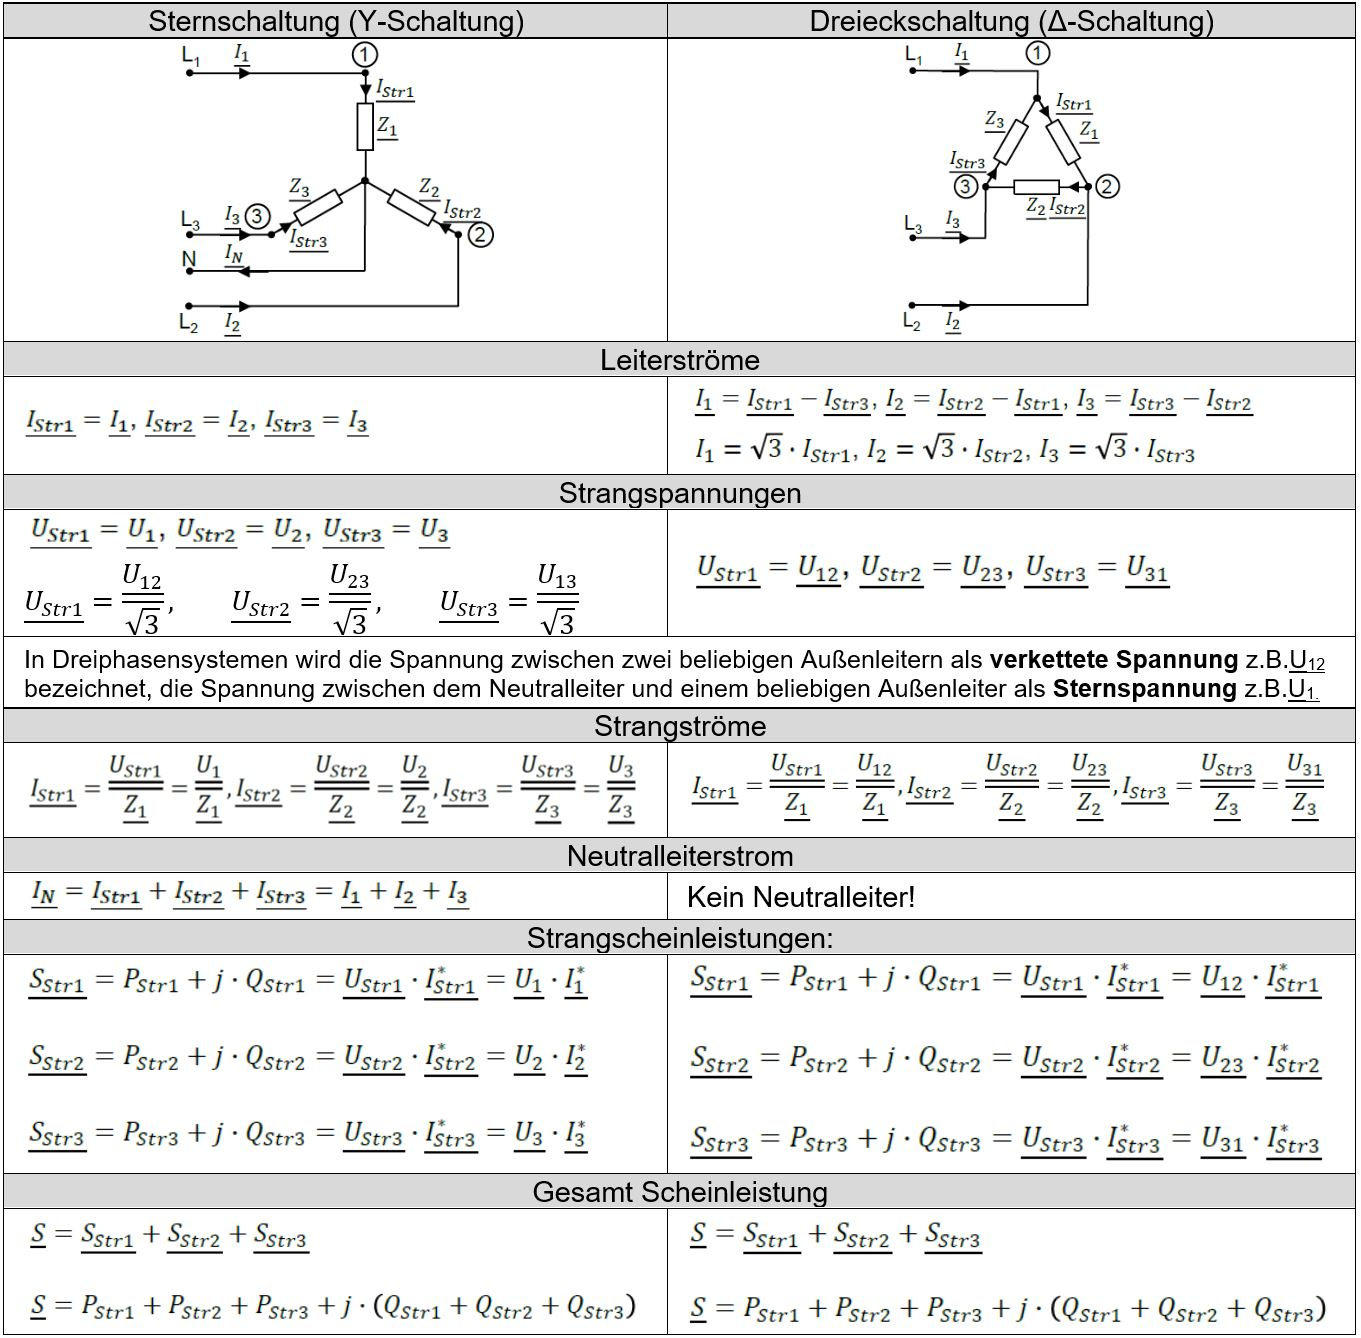
\includegraphics[scale = 0.8]{images/SternDreieck}
    \end{minipage}
    
%    \begin{minipage}[b]{0.4\linewidth}
%    	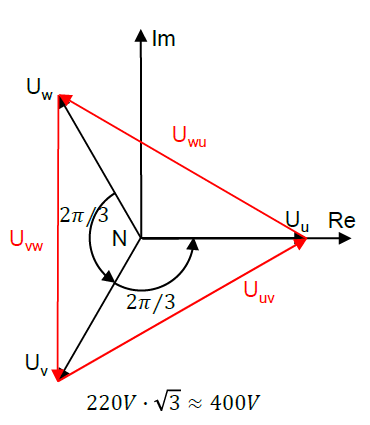
\includegraphics[width = 3.5cm]{images/Spg}
%    \end{minipage}
%    \begin{minipage}[b]{0.6\linewidth}
%    	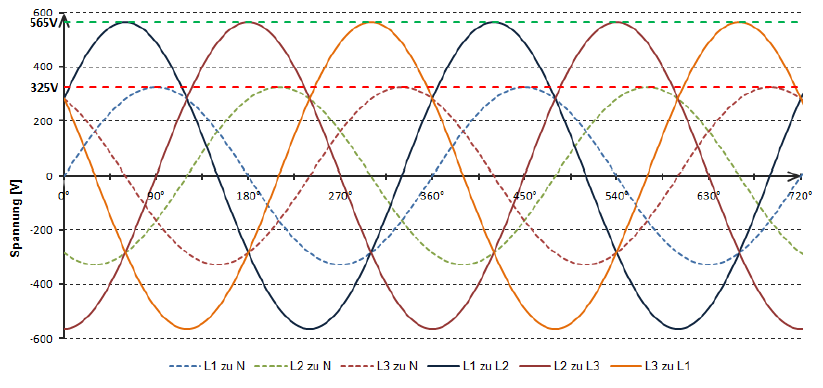
\includegraphics[width = 9cm]{images/Spg1}
%    \end{minipage}
    \clearpage
    \pagebreak

\section{Wicklungsschema Übung 4}
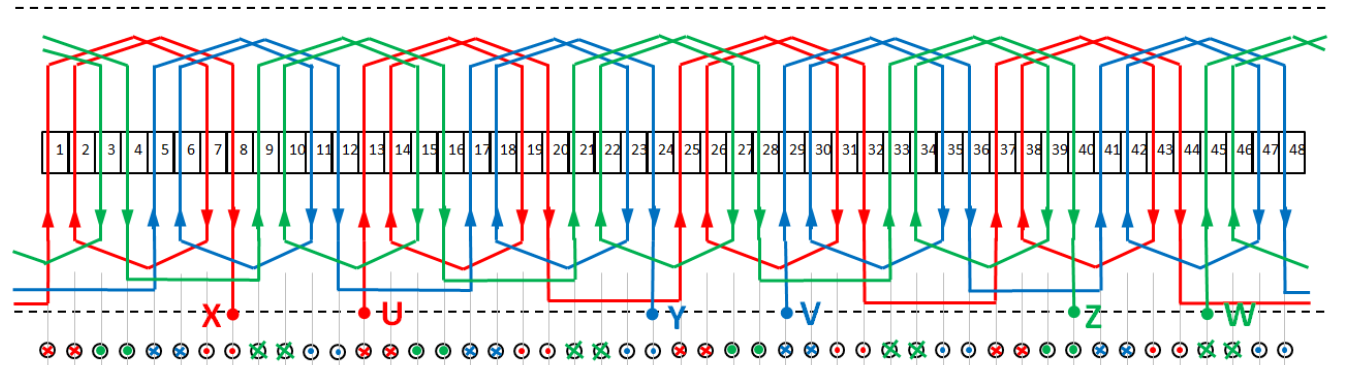
\includegraphics[scale = 0.5]{images/Wicklungsschema}
\subsection{Wichtige Formeln}
    \renewcommand{\arraystretch}{1}
\begin{tabular}{|C{0.3\textwidth}|P{0.3\textwidth}|P{0.3\textwidth}|}
	\hline
	\textbf{Drehzahl} &
    \[n = 60\cdot \dfrac{f}{p}\] &
    \vspace{0.1cm}n - Drehzahl [n] = $\dfrac{1}{min}$ \newline 
    f - Frequenz \newline
    p - Polpaarzahl 
    \\ \hline
	\textbf{Nutzahl} &
    \[ N = 2p\cdot q\cdot m\] &
    2p - Polzahl \newline 
    q - Nutzahl pro Phasenband \newline
    m - Strangzahl 
    \\ \hline						 
\end{tabular}

\subsection{Beispiel}%TODO Format und evt genauere erklärung
\begin{minipage}[b]{0.4\linewidth}	
"\,8-polig "\quad$\widehat{=}$ \quad 2p = 8 \newline
N = 48 \newline
m = 3 \newline
q = 2 \newline \newline
$i_{L1} = Real\{\underline{I_{L1}}\} = 0.5\cdot I_0$ \newline \newline
$i_{L2} = Real\{\underline{I_{L2}}\} = 0.5\cdot I_0$ \newline \newline
$i_{L3} = Real\{\underline{I_{L3}}\} = -1.0\cdot I_0$ 
\newline \newline
	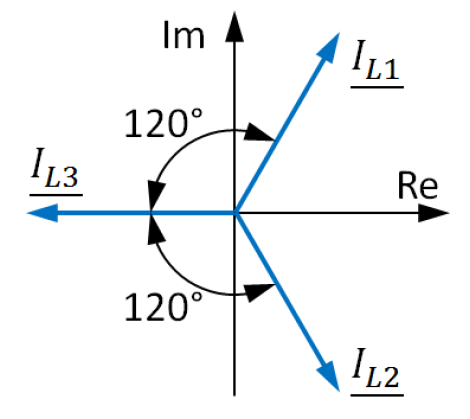
\includegraphics[scale = 0.4]{images/StromdreieckAGS}
\end{minipage}
\hspace{-0.5cm}
\begin{minipage}[b]{0.4\linewidth}
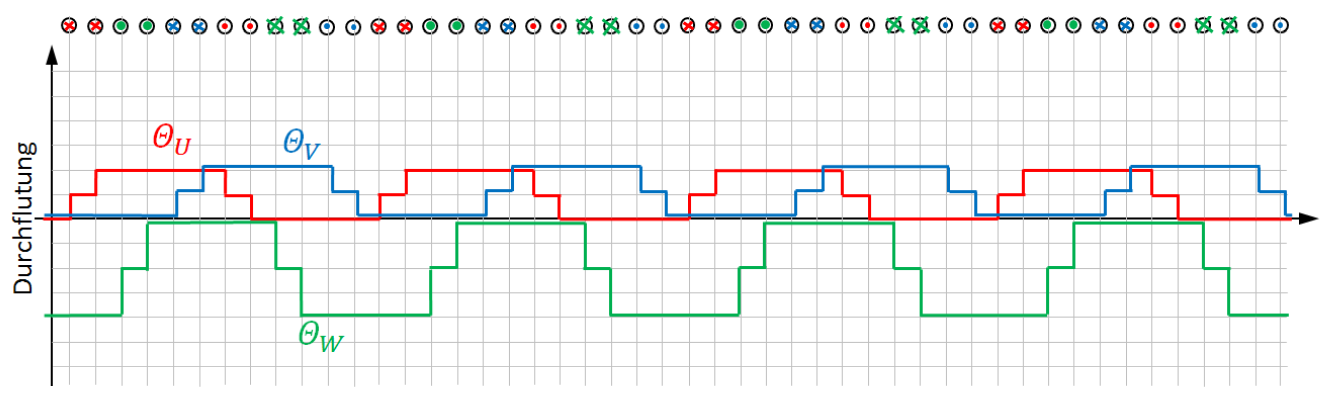
\includegraphics[scale = 0.35]{images/Durchflutung3} \newline
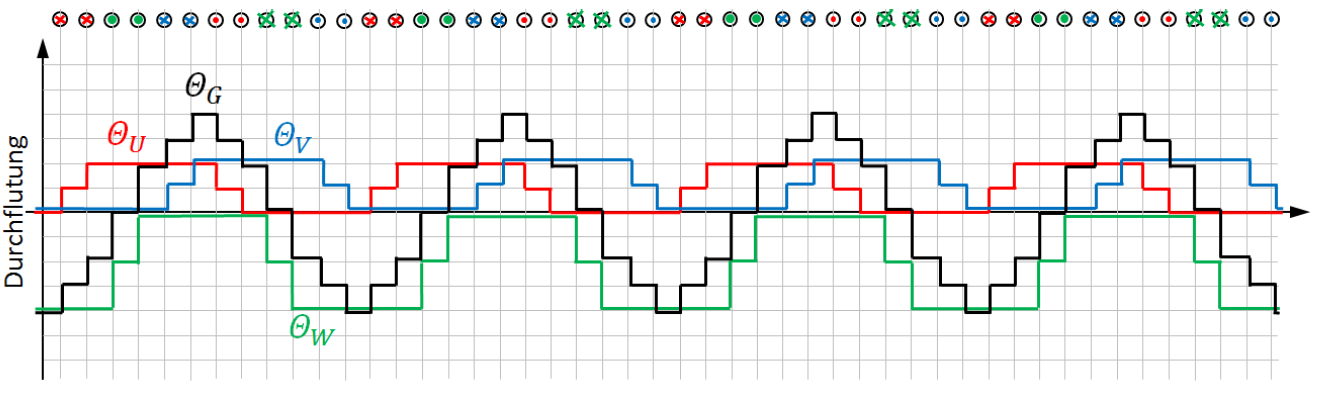
\includegraphics[scale = 0.35]{images/Durchflutung4} \newline

\end{minipage}
\clearpage
\section{Synchronmaschine}
    \renewcommand{\arraystretch}{2.5}
{\scriptsize \textcolor{green}{Vorteil}:
\begin{itemize} 
	\item sehr robust, elektrodynamisch, mechanisch und thermisch stabil
    \item Hoher Wirkungsgrad (80-90\%)
	\item Drehmoment einfach bestimmbar
	\item Einfache Konstruktion
	\item Man kann Blindleistung mit diesem Motor kompensieren
\end{itemize}
\textcolor{red}{Nachteil}:
\begin{itemize}
\item Anlaufstrom
\end{itemize}}
\subsection{Funktionsweise}
Das Drehfeld und der Rotor einer Synchronmaschine rotieren mit derselben Geschwindigkeit d.h. sind sie im Synchronlauf. \\
\textbf{Anwendung:} zur Umwandlung von mechanischer Energie in elektrische Energie.
\subsection{Aufbau und Wirkungsprinzip}
    \begin{minipage}[b]{0.5\linewidth}
    	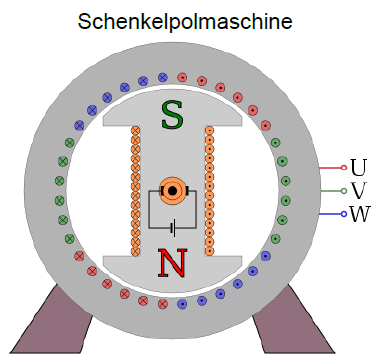
\includegraphics[width = 5cm]{images/Schenkelpolmaschine}
    \end{minipage}
    \begin{minipage}[b]{0.5\linewidth}
    	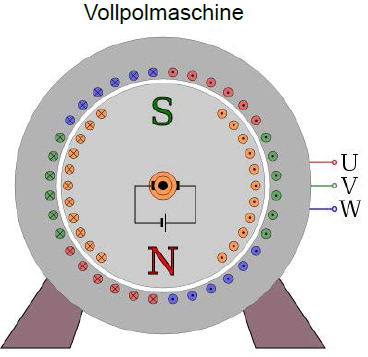
\includegraphics[width = 5cm]{images/Vollpolmaschine}
    \end{minipage}
    \begin{tabular}[b]{| C{0.4\linewidth} | C{0.4\linewidth} |}
    	\hline
    	\textbf{Schenkelpolmaschine} &
        \textbf{Vollpolmaschine}
        \\ \hline
        
    	\vspace{-0.7cm}
    	\begin{itemize}
    		\item Grössere Polpaarzahl
    		\item Kleinere Drehzahl
    		\item Wasserkraftwerk
    	\end{itemize} &
        \vspace{-0.7cm}
        \begin{itemize}
        	\item p = 1
        	\item Grössere Drehzahl
        	\item Wärmekraftwerke
        \end{itemize}
        \\ \hline
    \end{tabular}
    \\
    
    \begin{minipage}[b]{0.33\linewidth}
    	\raggedright
    	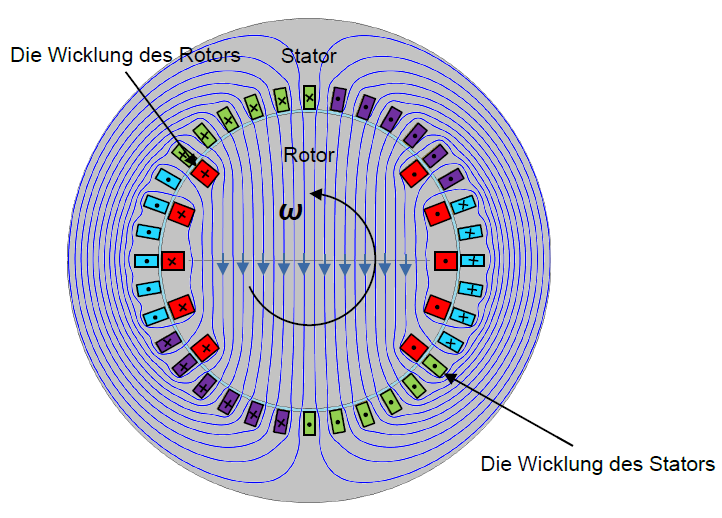
\includegraphics[width = 10cm]{images/AufbauSynchronmotor}
    \end{minipage}
    \clearpage
    \pagebreak

\subsection{Grundgleichungen}
    \begin{minipage}[b]{0.5\linewidth}
        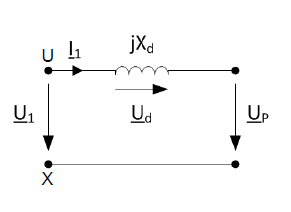
\includegraphics[width = 6cm]{images/Wicklung1}
    \end{minipage}
    \begin{minipage}[b]{0.5\linewidth}
        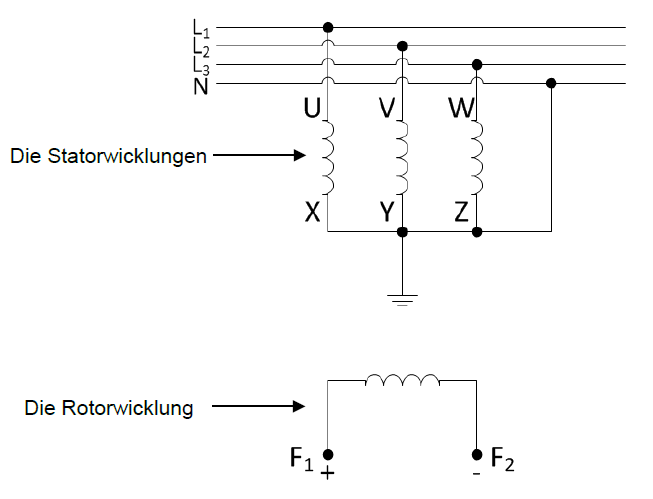
\includegraphics[width = 6.2cm]{images/Wicklungen}
    \end{minipage}
    \vspace{-1cm}
    \begin{longtable}[b]{| C{5cm}| P{8.5cm} | P{5 cm} |}
    	\hline
        \textbf{Strangspannung} 	&
        $\underline{U_1\!} = \underline{U_d\!} + \underline{U_P\!}$ &
        $U_P \, \widehat{=}$ der Polradspannung
        \\ \hline
        
        \textbf{Spulenspannung}	&
        $\underline{U_d} = jX_d\cdot \underline{I_1}$ &
        \\ \hline
        
        \textbf{Polradspannung} \newline (fiktive Hilfsgrösse) &
        $\underline{U_P} = \underline{U_P}\left(I_e\right)$ \newline\newline
        $\underline{U_P} = jX_h\cdot I_{e}\,'$  &
        $I_e \, \widehat{=}$ dem Erregerstrom \newline
        $I_e\,' \widehat{=}$ dem Erregerstrom umgerechnet auf die Statorseite
        \\ \hline
        
        \textbf{Synchronreaktanz} &
        $X_d = X_{\sigma 1} + X_h$ \newline \newline 
        $X_d = 2\pi f L_d$ \newline \newline
        $X_d = \dfrac{U_1}{\sqrt{3}\cdot I_K}$&
        $X_d \, \widehat{=} $ Synchronreaktanz \newline
        $X_{\sigma 1} \, \widehat{=}$ Streureaktanz des Stators \newline
        $X_h \, \widehat{=}$ der Hauptreaktanz \newline 
        $U_1\, \widehat{=}$ der Verketteten Spannung
        \\ \hline
        
        \textbf{Leistung} \newline
        \tabbild[scale=0.4]{images/SynchronKennlinie} &
        $\varphi = -\alpha - \dfrac{\pi}{2}$ \newline
        $\cos(\varphi) = -\sin(\alpha)$ \newline
       	$ (X_d \cdot I_1)^2=(\frac{U_1}{\sqrt{3}})^2+(\frac{U_p}{\sqrt{3}})^2 - 2\cdot \frac{U_1}{\sqrt{3}}\cdot \frac{U_p}{\sqrt{3}} cos(\delta) $ \newline \newline
       	$P_{Pro Strang} = U_1\cdot I_1\cdot cos(\varphi)$ \newline
        \textbf{Generatorbetrieb:} $\delta < 0$ \newline
        \textcolor{red}{d} = $-U_p\cdot\sin(\delta)$ \newline
        \qquad $= X_d\cdot I_1\cdot\sin(\alpha) = -X_d\cdot I_1\cdot\cos(\varphi)$ \newline \newline
        $P(\delta) = 3\dfrac{U_P\cdot U_1}{X_d}\cdot\sin(\delta)$ \newline \newline
        $P(\delta) = P_{mech}-P_V = \omega\cdot M - P_V$ \newline \newline
        \textbf{Motorbetrieb:} $\delta > 0$ \newline
        $P(\delta) = P_{mech} + P_V = \omega\cdot M + P_V$ &
        Polradwinkel $\delta =  \measuredangle (U_p, U_1)$  \newline \newline
        $U_P$ ist die Polradspannung, sie entspricht einer fiktiven Grösse! Sie kann wiederum durch ein Zeigerdiagramm bestimmt werden.
        \\ \hline
		\textbf{Erreger-Regulierkennlinien} & 
		$ \dfrac{I_e}{I_{e0}} = \sqrt{cos^2(\varphi) + \left(x\cdot\dfrac{I_1}{I_N}-sin(\varphi)\right)^2}$ & $I_e = f(I_1)$ \newline $cos(\varphi)$ gegeben \newline $I_1$ - gewünschter Netzstrom \newline Bezugswert $x = \dfrac{X_d}{X_N}$ 
		\\ \hline
		\textbf{mechanisches Moment} &  $P = \Omega\cdot M = \dfrac{\omega}{p}\cdot M$ & Gilt falls $P_V = 0$ 
		\\ \hline
	
	    \end{longtable}
    
    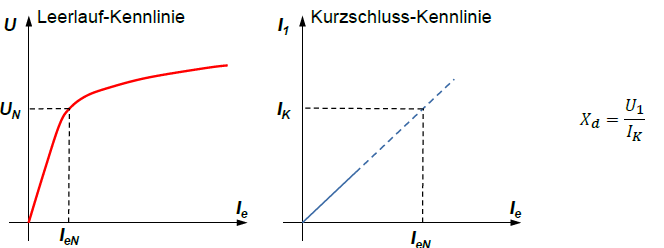
\includegraphics[scale = 0.8]{images/KennlinieSynchronmaschine}

\subsection{Zeigerdiagramm im Motorbetrieb}
    P > 0 und $\delta$ > 0 \newline \newline
    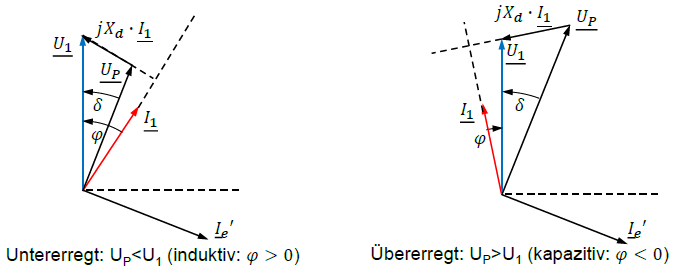
\includegraphics[width = 12 cm]{images/ZeigerdiagrammSynchronmaschine}

\subsection{Zeigerdiagramm im Generatorbetrieb}
    P < 0, $\delta$ < 0  \newline
    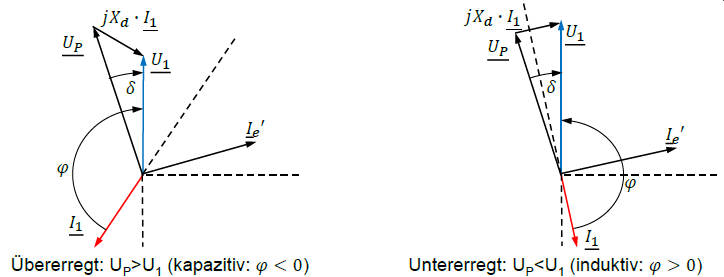
\includegraphics[width = 12 cm]{images/ZeigerdiagrammGeneratorbetrieb} \newline \newline
    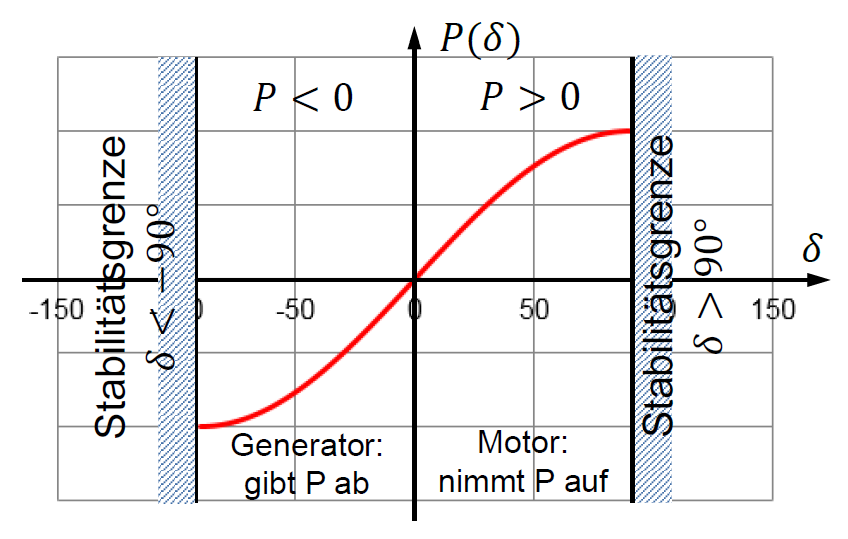
\includegraphics[scale = 0.4]{images/Stabilitaet}



\clearpage
\pagebreak

\section{Asynchronmotor}
Eigenschaften:
\begin{itemize}
    \item Meist verwendete Elektromotor
    \item Drehfekd wird durch den Ständer erzeugt
    \item Drehmoment entsteht durch den im Läufer induzierten Strom
\end{itemize}
\textcolor{green}{Vorteil}:
\begin{itemize}
	\item sehr einfacher Aufbau
	\item sehr robust und widerstandsfähig 
\end{itemize}
\textcolor{red}{Nachteil}:
\begin{itemize}
	\item Extrem hoher Anlaufstrom \newline
		$\Rightarrow$ dies wird vermindert mit der Stern-Dreieck-Umschalt-Methode \newline
        (Im Dreieck 3 Mal mehr Leistung im Dreieckbetrieb)
\end{itemize}

\subsection{Aufbau  Ständer}
    \begin{minipage}[b]{0.45\linewidth}
    	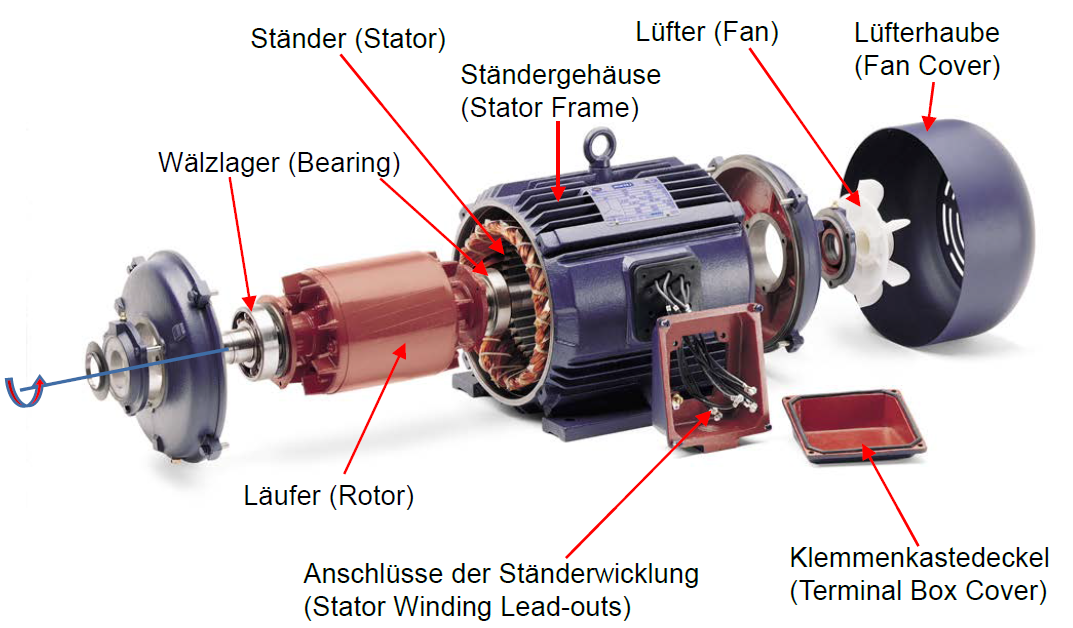
\includegraphics[scale = 0.3]{images/AsynchronmotorAufbau}
    \end{minipage}
    \begin{minipage}[b]{0.28\linewidth}
    	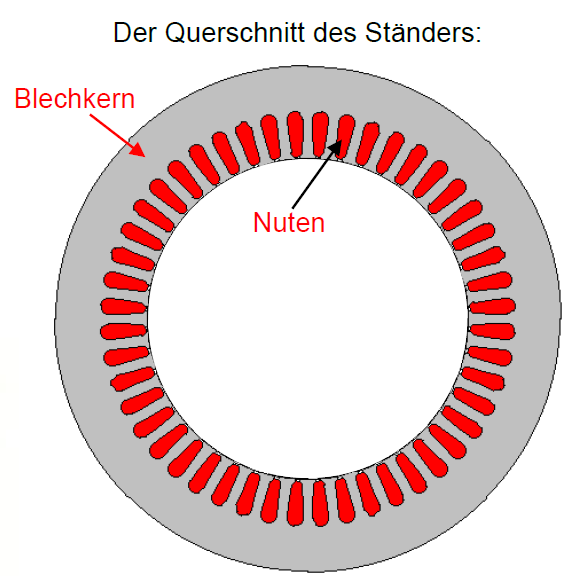
\includegraphics[scale = 0.3]{images/AQuerschnitt}
    \end{minipage}
    \begin{minipage}[b]{0.33\linewidth}
    	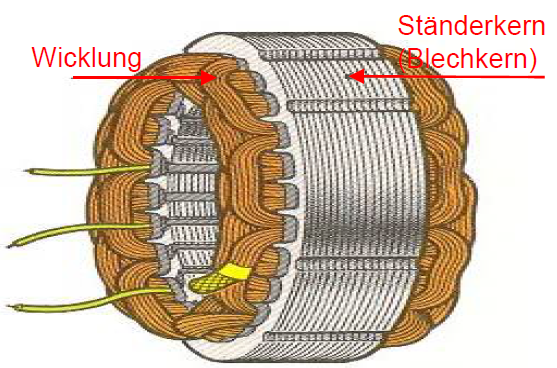
\includegraphics[scale = 0.4]{images/AsynchronmotorStaenderkern}
    \end{minipage}\\
    \subsection{Aufbau Läufer}
    \begin{minipage}[b]{0.5\linewidth}
    	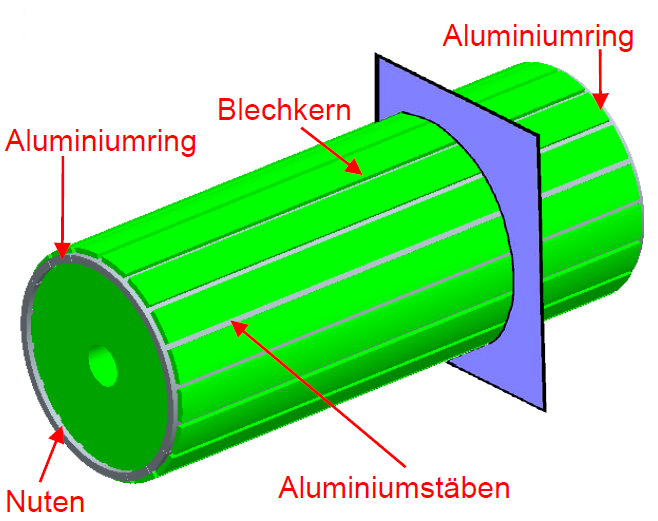
\includegraphics[scale = 0.4]{images/AsynchronRotor}
    \end{minipage}
    \begin{minipage}[b]{0.5\linewidth}
    	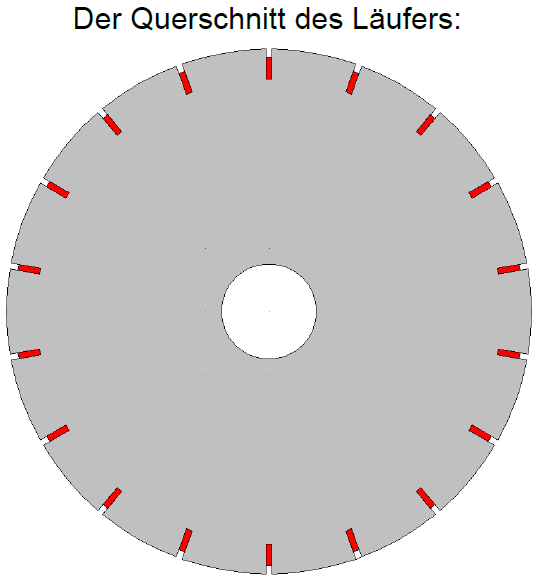
\includegraphics[scale = 0.4]{images/QuerschnittAsynchronrotor}
    \end{minipage}
    \\ \\
    Wirbelströme im Eisen entstehen durch die Induktion des Rotors in den Stator \newline
    $\Rightarrow$ Stator erwärmt sich.\newline
    Durch den Rillenaufbau des Stators können diese Wirbelströme bzw. die Temperaturansteigung minimiert werden.
    \\
    Schlupf $\widehat{=}$ der Abweichung zu der Synchronen Drehzahl 
    \clearpage
    \pagebreak

\subsection{Formeln Läufer}
    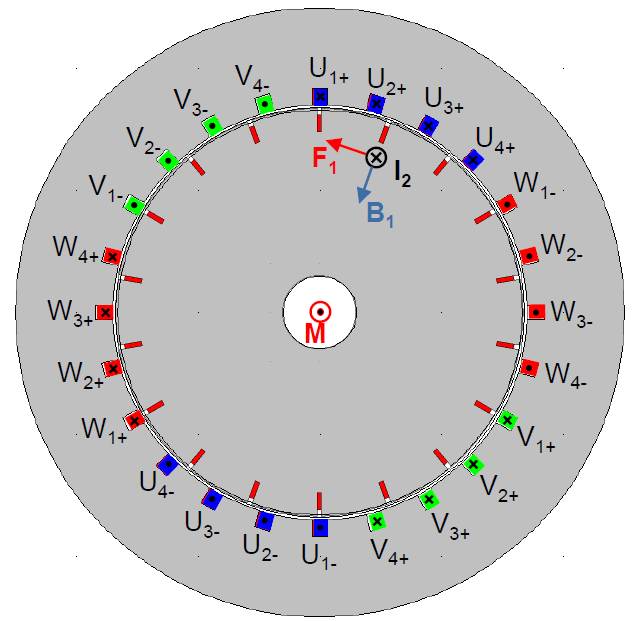
\includegraphics[scale = 0.4]{images/QuerschnittAmotor}
    \\ \\
    \begin{longtable}{| p{.25\textwidth} | p{.40\textwidth} | p{.30\textwidth} |}
    	\hline
    	\textbf{Induzierte Spannung} &
        \[ U_i = 4.44\cdot f\cdot w\cdot\xi\cdot\phi \] &
        f $\widehat{=}$ Frequenz \newline
        w $\widehat{=}$ Windungszahl \newline
        $\xi$ = Wicklungsfaktor \newline
        $\phi$ = Magnetischer Fluss
        \\ \hline
        
        \textbf{Elektromagnetische Kraft}	&
        \begin{equation*} \vec{F_2} = I_2\cdot\vec{I_2}\times\vec{B_1}\end{equation*} &
        \\ \hline
        
        \textbf{Mech. Drehmoment}	&
        \begin{equation*}\vec{M_2} = \vec{r_2}\times\vec{F_2}\end{equation*}&
        \\ \hline
        
        \textbf{Relativdrehzahl}&
        \[ n_1= \frac{f_1}{p}\]
        \[ n_2=n_1 - n \]&
        n = Drehzahl des Läufers \newline
        $n_1$ = Synchrondrehzahl \newline
        $ n_2 $ = Relativdrehzahl
        \\ \hline
        
        \textbf{Schlupf}&
        \[ s= \frac{n_2}{n_1}=\frac{n_1-n}{n_1}=\frac{f_2}{f_1} \]&
        $ f_1 $ = Frequenz Drehfeld \newline
        $ f_2 $ = Frequenz Anker \newline
        Synchroner Lauf: s = 0 \newline
        Stillstand: s = 1
        \\ \hline 
        
        \textbf{Induzierter Strom des Läufers}&
         \[ I_2 = \frac{U_{i20}}{\sqrt{R_2^2+X_{2\sigma}^2}} \]&
         \\ \hline
        
        \textbf{Stillstand}\newline
         s = 1 \newline
        $ f_2 = f_1 $ &
        \[ I_2 = I_{2max} = \frac{U_{i20}}{\sqrt{(R_2/2)^2+X_{2\sigma^2}}} \]&
         \newline
        \tabbild[scale=0.3]{images/FlussStillstand}       
        \\ \hline
        
         \textbf{Synchronlauf} \newline
          s = 0 \newline
         $ f_2 = 0 $&
         \[ I_2 = I_{2max} = 0\]&
          \newline
         \tabbild[scale = 0.3]{images/FlussSynchron}
         \\ \hline

        
        \textbf{Verluste Drehmoment}\newline
        \tabbild[scale = 0.3]{images/PVerluste}&
        \[ P_{D1}=P_m+P_{C22} \]
        \[ P_{D1}=2\cdot\pi\cdot n_1\cdot M \quad
         P_m = 2\cdot\pi\cdot n\cdot M \]
        \[ M = \frac{1}{2 \pi n_1}\frac{P_{Cu2}}{s} \]&
         $ P_1 $ - primäre Netzleistung \newline
         $ P_{Cu} $ - Ohmsche Verluste \newline
         $ P_{Fe} $ - Blechkernverluste \newline
         $ P_{D1} $ - Drehfeldleistunf \newline
         $ P_m $ - mechanische Leistung \newline
         $ P_r $ - Reibungsverluste und Lüftung \newline
         $ P_m ' $ - mech. Nutzleistung \newline
         M - Drehmoment
        \\ \hline
        
        \textbf{Funktion Drehmoment} \newline
        \tabbild[scale = 0.4]{images/FunktionDrehmoment}&
        \[ M=\frac{1}{2\pi n_1}\frac{\textcolor{blue}{P_{Cu2}}}{s} \]
        \[= \frac{\textcolor{blue}{q_2}}{2\pi n_1}\cdot \textcolor{green}{I_2^2}\cdot\frac{\textcolor{blue}{R_2}}{s} \]
        \[= \frac{q_2}{2\pi n_1}\textcolor{green}{\frac{U_{i20}^2}{(R_2/s)^2+X_{2\sigma}^2}}\frac{R_2}{s} \]&
        \textcolor{blue}{M-Kennlinie} \newline
        \textcolor{yellow}{Motorbetrieb} \newline
        \textcolor{green}{Generator-Betrieb}
        \\ \hline
        
        \textbf{Anlauf} \newline
        \tabbild[scale=0.4]{images/ASMAnlauf}&
        \[ M=\frac{q_1}{2\pi n_1}\cdot \frac{U_1^2}{(R_2'/s)^2+X_{2\sigma}^2}\cdot\frac{R_2'}{s} \]
        \[ s_K=\frac{R_2'}{X_{2\sigma}'} \]
        \[ M_K= \frac{q_1}{4\pi n_1}\cdot\frac{U_1^2}{X'_{2\sigma}} \]&
        \\ \hline
        
        \textbf{Klosssche Gleichung}&
        \[ \frac{M}{M_K}=\frac{2}{\frac{s}{s_K}+\frac{s_K}{s}} \]&
        \\ \hline        
              
    \end{longtable}
    
\subsection{Model der Asynchromaschine}
    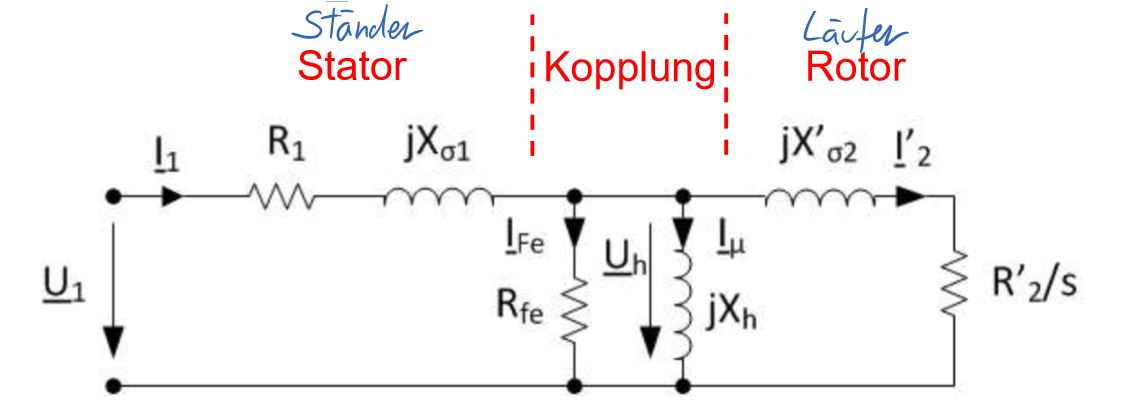
\includegraphics[scale = 0.6]{images/ModelASM}
    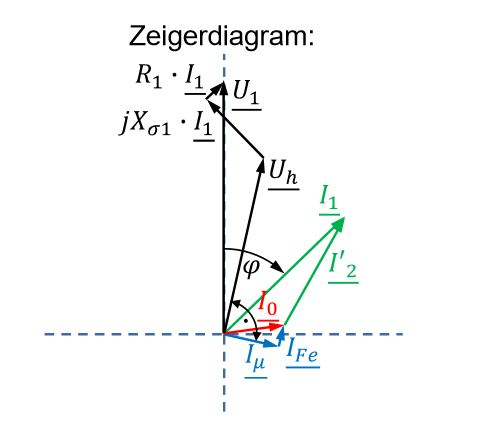
\includegraphics[scale = 0.7]{images/ModelASMZeiger}
    %TODO Kennlinie ASM S27

    \begin{longtable}{| p{.55\textwidth} | p{.45\textwidth}|}
        \hline
        \textbf{Grundgleichungen:}\newline
        \[ \underline{I_1}= \underline{I_{FE}}+\underline{I_\mu}+\underline{I'_2} \]
        \[ \underline{U_1}= R_1 \cdot \underline{I_1}+jX_{\sigma 1}\cdot \underline{I_1}+ \underline{U_h} \]
        \textbf{Übersetzungsverhältnis:}\newline
        \[ u=\frac{N_1 \cdot k_{w1}}{N_2 \cdot k_{w2}}\]
        \[ \underline{I'_2}=\underline{I_2 \cdot u} \]
        \[ R'_2 = R_2 \cdot u^2 \]&
        N = Windungszahl \newline
        $ k_w $ = Wicklungsfaktor \newline
        $ R_1, X_{\sigma 1} $= Widerstand und Streureaktanz des Stators \newline
        $ R_2, X_{\sigma 2} $= Widerstand und Streureaktanz des Rotors \newline
        $ R_{fe} $= Eisen-Verlustewiderstand \newline
        $ X_h $= Hauptreaktanz \newline
        $ U_h $= innere Spannung \newline
        $ I_\mu $= Magentisierungsstrom
        \\ \hline      
        
        \textbf{Leerlauf} \newline
        \tabbild[scale=1]{images/ASMLeerlaufZeiger}&
         \newline
        \tabbild[scale=1.3]{images/ASMLeerlauf}
        \\
        
        \[ \underline{I_0}=\underline{I_{FE}} + \underline{I_\mu} \]
        \[ cos(\varphi_0)= \frac{P_0}{U_0 \cdot I_0} \]
        \[ R_{FE}=\frac{U_0}{I_{FE}}=\frac{U_0}{I_0 \cdot cos(\varphi_0)} \]
        \[ X_h = \frac{U_0}{I_\mu}=\frac{U_0}{I_0 \cdot sin(\varphi_0)} \]&
         \textbf{Im Leerlauf wird die Asynchronmaschine an der Welle nicht belastet.} \newline
        \[ R_1 << R_{FE} \qquad X_{\sigma 1} << X_h\]
        \\ \hline
        
        \textbf{Kurzschluss} \newline
        \tabbild[scale=1]{images/ASMKurzschlussZeiger}&
         \newline
        \tabbild[scale=0.8]{images/ASMKurzschluss}
        \\
        
        \[ cos(\varphi_K)= \frac{P_K}{U_K \cdot I_K} \]
        \[ R1 + R'_2 = \frac{U_R}{I_K} = \frac{U_K \cdot cos(\varphi_k)}{I_K} \]
        \[ X_{\sigma 1}+ X'_{\sigma 2}= \frac{U_X}{I_K}=\frac{U_K \cdot sind(\varphi_K)}{I_k} \]
        &
         \textbf{Im Kurzschluss wird der Rotor der Asynchronmaschine blockiert.} \newline
         \[ R_1 << R_{FE} \qquad X_{\sigma 1} << X_h\]
         \\ \hline
         
         \textbf{4Q- Umrichter} \quad FU = Frequenzumrichter\newline
         \tabbild[scale=0.8]{images/4QSchema}&
          \newline
         \tabbild[scale=0.8]{images/4QMn}
         \\ \hline
         
        
        
        
    \end{longtable}
    
    \clearpage
    \pagebreak

\section{Schrittmotor}
\subsection{Merkmale}
    \begin{itemize}
        \item Der Schrittwinkel hängt vom Aufbau der Maschine ab und kann zwischen 0.6° und 15° sein.
        \item moderne Arten der Schrittmotoren
        \item Drehmoment bis zu 5 Nm
        \item Werden im unteren leistungsbereich eingesetzt
        \begin{itemize}
            \item Reluktanz-SM
            \item Hybrid-SM
            \item Permanentmagnet-SM
        \end{itemize}
    \end{itemize}
    \textcolor{green}{Vorteil}:
    \begin{itemize}
        \item hoher Wirkungsgrad
        \item gute statische und dynamische Eigenschaften
        \item Kostengünstig
        \item praktisch nicht überlastbar
    \end{itemize}

\subsection{Reluktanz-SM}
    \begin{longtable}{| p{.40\textwidth} | p{.60\textwidth} |}
        \firsthline
        \textbf{Aufbau} \newline
        \tabbild[scale=0.5]{images/AufbauReluktanzSM.JPG} &	
        \newline
        Stator-Zähne: $ SZ_1, SZ_2, SZ_3, SZ_4$ \newline
        Stator-Wicklung: $ SW_1, SW_2, SW_3, SW_4 $ \newline
        Rotor-Zähne: $ RZ_1, RZ_2$
        \\ \hline
        
        \textbf{Wirkungsprinzip} \newline
        \tabbild[scale=0.45]{images/WirkPrinzReluktanzSM.JPG}&
        \newline
        Die magentische Reluktanzkraft ist immer anziehend \newline
        $\Rightarrow$ veruscht den Luftspalt zu verkleinern.
        \\ \hline
        
         \newline
        \tabbild[scale=0.5]{images/FLWirkPrinzReluktanzSM.JPG}&
        \newline
        Die Spule $ SW_1 $ ,$ SW_3 $ sind an die Quelle angeschlossen. \newline
        Das magnetische Feld der ersten zwei Spulen wird erzeugt. \newline
        Die Reluktanzkraft wirkt auf den Rotor um die Lluftspalte zu verringern. \newline
        Das mechanische Moment wird erzeugt.
        %\\ \hline
        
        %TODO Passende Grafik einfügen ca S.24 Vorlesung Aktive Wicklungen beachten.
        %Evt mit \multicolumn formatieren
%            \tabbild[scale=0.35]{images/ReluktanzSM1.JPG}\vline
%            \tabbild[scale=0.35]{images/ReluktanzSM2.JPG}&
%            \tabbild[scale=0.35]{images/ReluktanzSM3.JPG}\vline
%            \tabbild[scale=0.35]{images/ReluktanzSM4.JPG}
%            \\ \hline
%            
%            \tabbild[scale=0.35]{images/ReluktanzSM11.JPG}\vline
%            \tabbild[scale=0.35]{images/ReluktanzSM21.JPG}&
%            \tabbild[scale=0.35]{images/ReluktanzSM3.JPG}\vline
%            \tabbild[scale=0.35]{images/ReluktanzSM41.JPG}
        
        \\ \lasthline
    \end{longtable}

\subsection{Permanentmagnet-SM}
    \begin{longtable}{| p{.35\textwidth} | p{.60\textwidth} |}
        \firsthline
        \textbf{Aufbau} \newline
        \tabbild[scale=0.5]{images/AufbauPMagnetSM.JPG} &	
        \newline
        Stator-Zähne: $ SZ_1, SZ_2, SZ_3, SZ_4$ \newline
        Stator-Wicklung: $ SW_1, SW_2, SW_3, SW_4 $ \newline
        Rotor-Zähne: $ RZ_1, RZ_2$ 
        \\ \hline
        
        \textbf{Grundgleichnung} & %TODO Format 3-Spalten
        Stator-Zahnzahl: $  MZ_s $  \newline
        Rotor-Zahnzahl: $ Z_R $  \newline
        Stator-Winkel: $ \alpha_S=\frac{2\pi}{Z_s}$ \quad [rad]  \newline
        Rotor-Winkel: $ \alpha_R=\frac{2\pi}{Z_R}$ \quad [rad]  \newline
        Vollschritt-Winkel: $ \alpha_0 = \alpha_R - \alpha_S $ \newline
        Der Vollschrittwinkel berzeichnet die Bewegung des Rotors pro Einzel-Steuerimpuls. \newline
        Strangzahl: $ m= \frac{Z_s}{Z_S - Z_R} $\newline
        Schrittzahl: $ N_p = \frac{2\pi}{\alpha_0}  $\newline
        Steuerfrequenz: $ f_s = N_p * n $\quad $ (n=[s^-1]) $
        \\ \hline
        
         \newline
        \tabbild[scale=0.4]{images/IndukdqSM.JPG}&
        \newline
        \textcolor{red}{wahre Induktivität} \newline
        \textcolor{blue}{lineare Annäherung} \newline \newline
        N = Windungszahl Statorstrang \newline
        $ A_z $ = Zahnfläche \newline
        $ \delta_{d} = \delta_{q}$ = Höhe des Luftspalts
        \\ \hline            
        %TODO w_zu ist die breite der Zahnüberlappung in q position??ubung 7 
        d-Achse Parallel\newline
        \tabbild[scale=0.6]{images/StatordSM}&
        \[ L_d = \frac{\varPsi_{md}}{I_1}
        =2N \frac{\varPhi_{md}}{I_1}
        =2N\frac{B_{\delta d}A_z}{I_1}
        =\mu_0 2N\frac{2NI_1A_z}{2\delta_d I_1} \]
        \[\quad =\mu_0 2N^2\frac{A_z}{\delta_d} 
         = \mu_0 2N^2\frac{L \cdot w_s}{\delta_d} \]
        \\ \hline
                   
        q-Achse Parallel\newline
        \tabbild[scale=0.6]{images/StatorqSM}&
        \[ L_q = \frac{\varPsi_{mq}}{I_1}
        =2N \frac{\varPhi_{mq}}{I_1}
        =2N\frac{B_{\delta q}A_z}{I_1}
        =\mu_0 2N\frac{2NI_1A_z}{2\delta_q I_1}\]
        \[\quad =\mu_0 2N^2\frac{A_z}{\delta_q} 
        = \mu_0 2N^2\frac{L \cdot w_{zu}}{\delta_q} \]
        
        \\ \lasthline
    \end{longtable}
\subsection{V11-12 S43}
\begin{longtable}{| p{.35\textwidth} | p{.60\textwidth} |}
    \firsthline
    \newline
    \tabbild[scale=0.6]{images/StatordqSM1}&
    $ \varPhi_m(y_r,i) = L(y_r(t)) \cdot i(t) $\newline
    \[ u_{Statorkreis}(t)=R\cdot i(t) + \frac{\diff\varPhi_m}{\diff t}(t) = R \cdot i(t) + \frac{\diff}{\diff t}\left[L(y_r(t))\cdot i(t) \right]\] 
    \[\qquad = R \cdot i(t) + \frac{\diff L}{\diff  y_r} (y_r)\cdot \frac{\diff  y_r}{\diff t} i(t) +L(y_r)\cdot \frac{\diff i}{\diff t}(t)\]
    \[ p_{Statorkreis}(t)=u(t) \cdot i(t) = R\cdot i^2(t)+\frac{\diff L}{\diff Y_r}(y_r)\cdot \omega_r\cdot i^2(t)+L\cdot i(t)\cdot \frac{\diff i}{\diff t}(t) \]
    \\ \hline
    
    \textbf{Elektrische Leistung des Stators}&
    \[ p(t) = R \cdot i^2(t) + \frac{\diff L}{\diff y_r}\cdot \omega_r \cdot i^2(t) + L \cdot i(t) \cdot\frac{\diff i}{\diff t}(t) \]
    \[=p_{Cu}(t)+\frac{\diff w_m}{\diff t}(t)+\frac{1}{2}\cdot \frac{\diff L}{\diff y_r}(y_r)\cdot \omega_r \cdot i^2(t) \]
    \\ \hline
    
    \textbf{Zeitableitung magnetischer Energie}&
    \[ w_m(t) = \frac{1}{2} \cdot L(y_r) \cdot i^2(t) \Rightarrow \frac{\diff }{\diff t} \left( \frac{1}{2} \cdot L(y_r) \cdot i^2(t) \right) \]
    \[=\frac{1}{2}\cdot \frac{\diff L}{\diff y_r}(y_r)\cdot\omega_r \cdot i^2(t) + L \cdot i(t) \cdot \frac{\diff i}{\diff t}(t) \]
    \\ \hline
    
    \textbf{Rotorleistung}&
    \[ p_\delta(t)= \frac{1}{2}\cdot \frac{\diff L}{\diff y_r}(y_r)\cdot \omega_r \cdot i^2(t) \]
    \\ \hline
    
    \textbf{Motormoment}&
    \[ m_M(t)=\frac{p_\delta}{\omega_r}(t)=\frac{1}{2}\cdot\frac{\diff L}{\diff y_r}(y_r)\cdot i^2(t) \]
    \\ \hline
    
    \textbf{Mototrmoment Linerar}&
    \[ M_M = \frac{1}{2}\frac{L_d - L_q}{\alpha_0}I_1^2 \]
    \\ \hline
    
    \newline
    \tabbild[scale=0.7]{images/IndukdqSMY}&
    \newline
    \tabbild[scale=0.7]{images/MomentdqSMY}
    \\ \hline
    
    \textbf{Betriebsverhalten}\newline
    \[ J_g \frac{\diff \omega_r}{\diff t}= J_g \frac{\omega_s - \omega_1}{T_s} = M_M - M_L \] \newline
    $ \omega_s = 2\pi\frac{n_s}{60}=2\pi\frac{f_s}{N_p}=\alpha_0 f_s $&
    $ J_g $ = Motorbezogenes Trägheitsmoment \newline
    $ M_M $ = Motorbezogenes Drehmoment \newline
    $ M_L $ = Lastmoment \newline
    $ \omega_s $ = Kreisgeschwindigkeit Statorfeld \newline
    $ \omega_1 $ = Kreisgeschwindigkeit des Rotors \newline
    $\Rightarrow  \omega_1 = 0 \Rightarrow$ Motor im Stillstand \newline
    \\ \hline
    
    \textbf{Lastmoment} \newline
    \[ M_L(f_s,\omega_1) = M_M -J_g\frac{\omega_s}{T_s}+J_g\frac{\omega_1}{T_s}\]
    \[=M_m -J_g\alpha_0f_s^2+J_g\omega_1f_s \]
    \[ f_{AG}=\sqrt{\frac{M_M}{J_R \cdot \alpha_0}} \]&
    \newline
    $ F_s = \frac{1}{T_s} $ = Schaltfrequenz\newline
    $ \omega_1 $ = Anfangsgeschwindigkeit \newline
    \\ \hline
    
    \textbf{Anlaufkennlinie}\newline
    \tabbild[scale=0.4]{images/AnlaufkennlinieSM.JPG}&
    $ f_{AG} $ = Anlaufgrenzfrequenz \newline
    $ f_{BG} $ =  Betriebsgrenzfrequenz
    \\ \hline
    
\end{longtable}


    

\clearpage
\pagebreak     
\section{Vergleich der Elektrischen Maschinen}

\begin{longtable}{| p{.30\textwidth} | p{.60\textwidth} |}
    \hline
    
    \textbf{Aufbau}&
     \newline
    \tabbild[scale=0.55]{images/VergleichMotor}
    \\ \hline
    
    \textbf{Komplexität des Aufbaus}&
     \newline
    \tabbild[scale=0.5]{images/VergleichMotorKomplex}
    \\ \hline
    
    \textbf{Kosten}&
     \newline
    \tabbild[scale=0.5]{images/VergleichMotorKosten}
    \\ \hline
    
    \textbf{Wirkungsgrad}&
     \newline
    \tabbild[scale=0.5]{images/VergleichMotorWirkungsgrad}
    \\ \hline
    
    \textbf{Anpassungsfähigkeit}&
     \newline
    \tabbild[scale=0.5]{images/VergleichMotorAnpassung}
    \\ \hline
    
    \textbf{Anlaufstrom}&
     \newline
    \tabbild[scale=0.5]{images/VergleichMotorAnlaufstrom}
    \\ \hline
    
    \textbf{Anlaufmoment}&
     \newline
    \tabbild[scale=0.5]{images/VergleichMotorAnlaufmoment}
    \\ \hline
    
    \textbf{Drehzahlregelung}&
     \newline
    \tabbild[scale=0.5]{images/VergleichMotorDrehzahl}
    \\ \hline
    
    \textbf{Anwendungsbereich}&
     \newline
    \tabbild[scale=0.5]{images/VergleichMotorAnwendung}
    \\ \hline   
\end{longtable}   
\clearpage
\pagebreak
\subsection{Auswahl Flowchart}

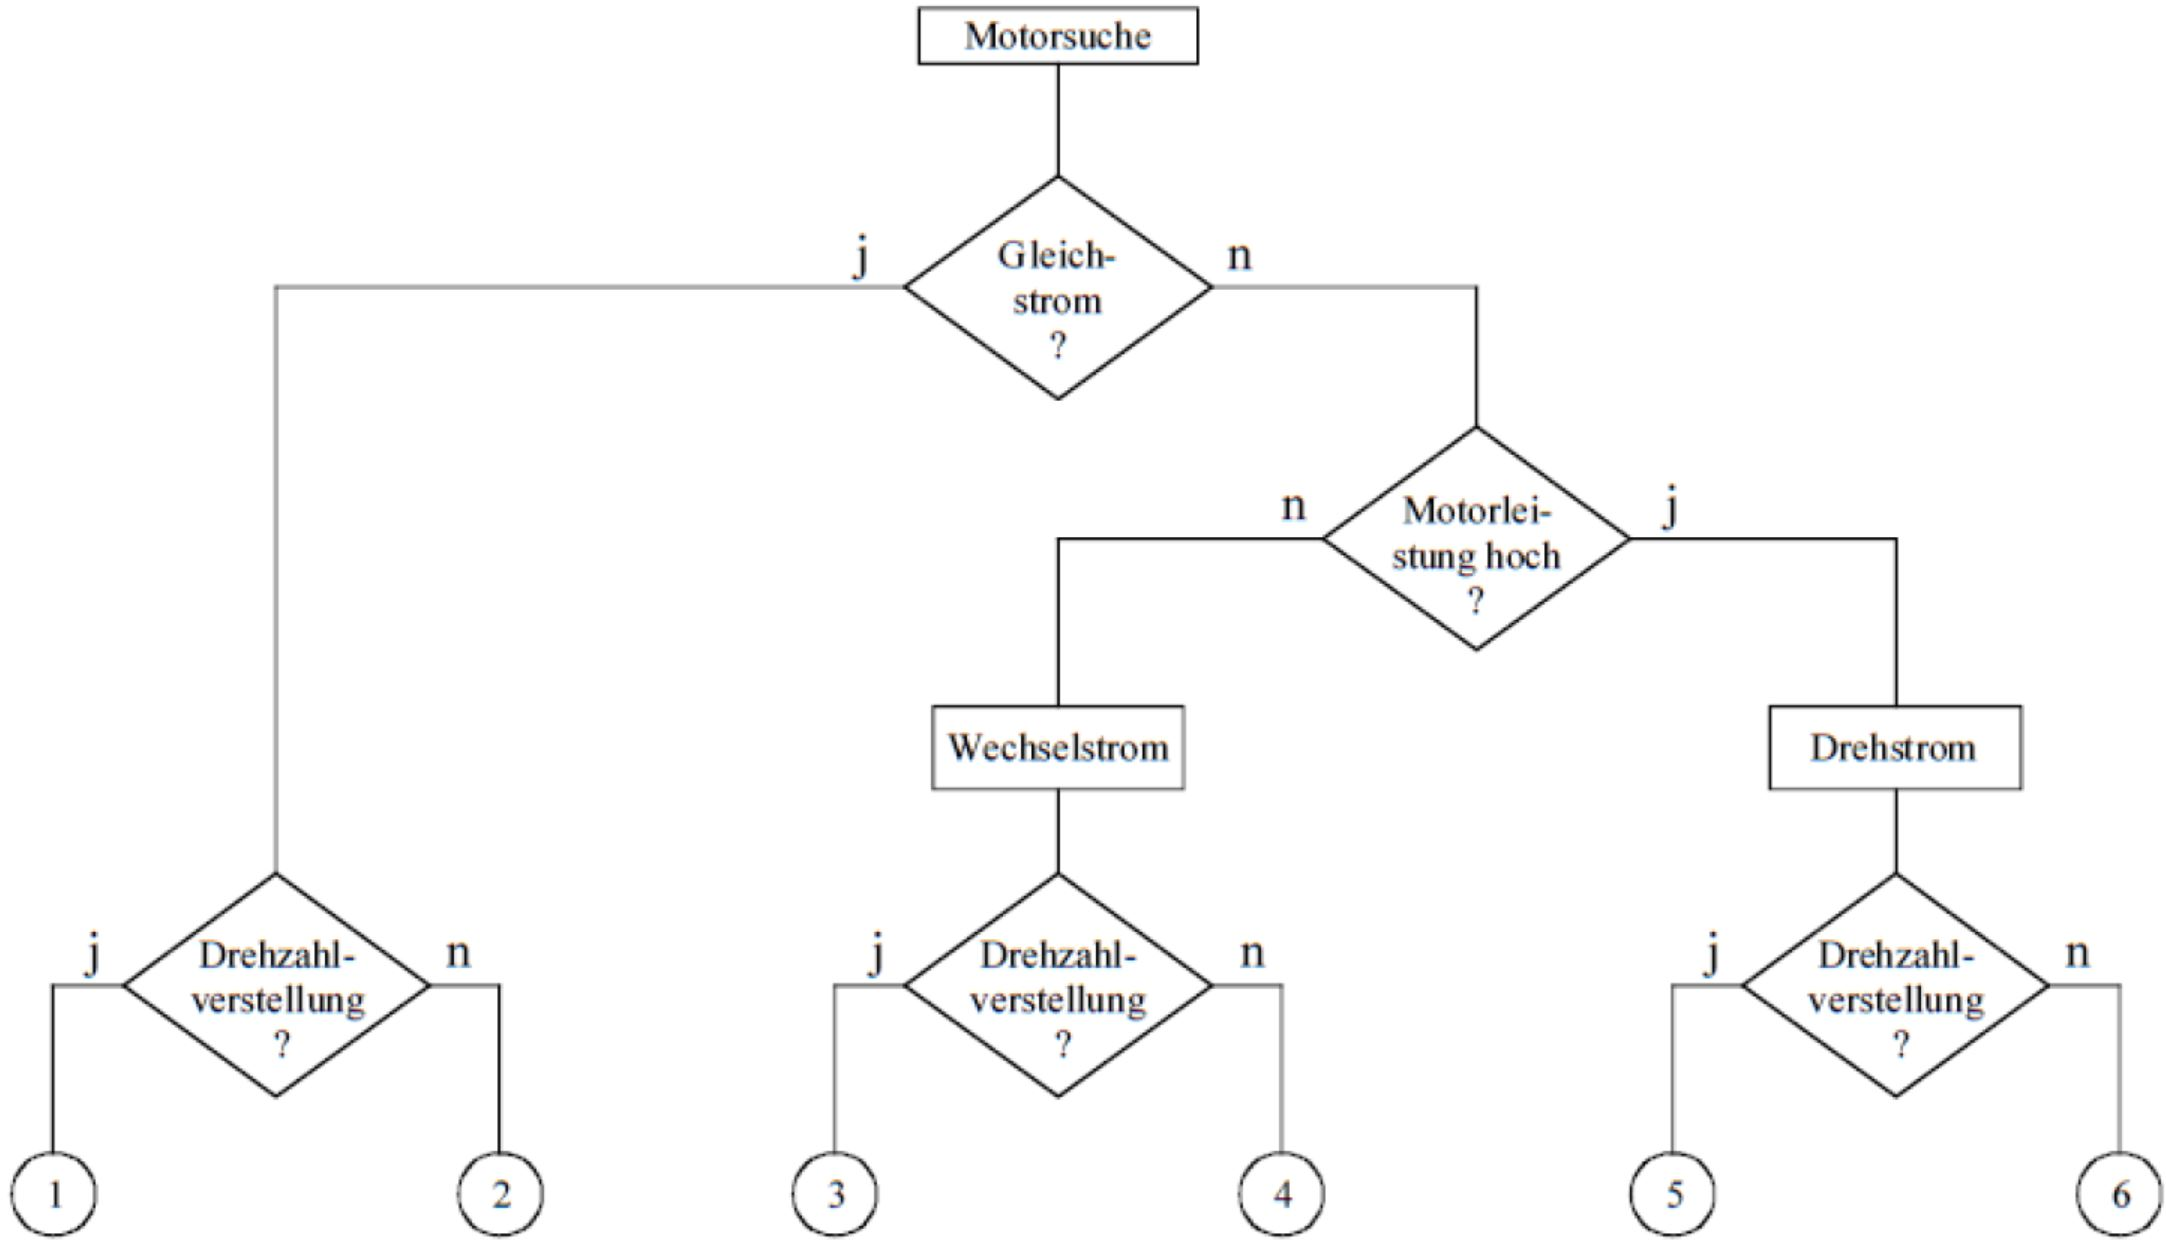
\includegraphics[scale=1]{images/Motorauswahl}
\\
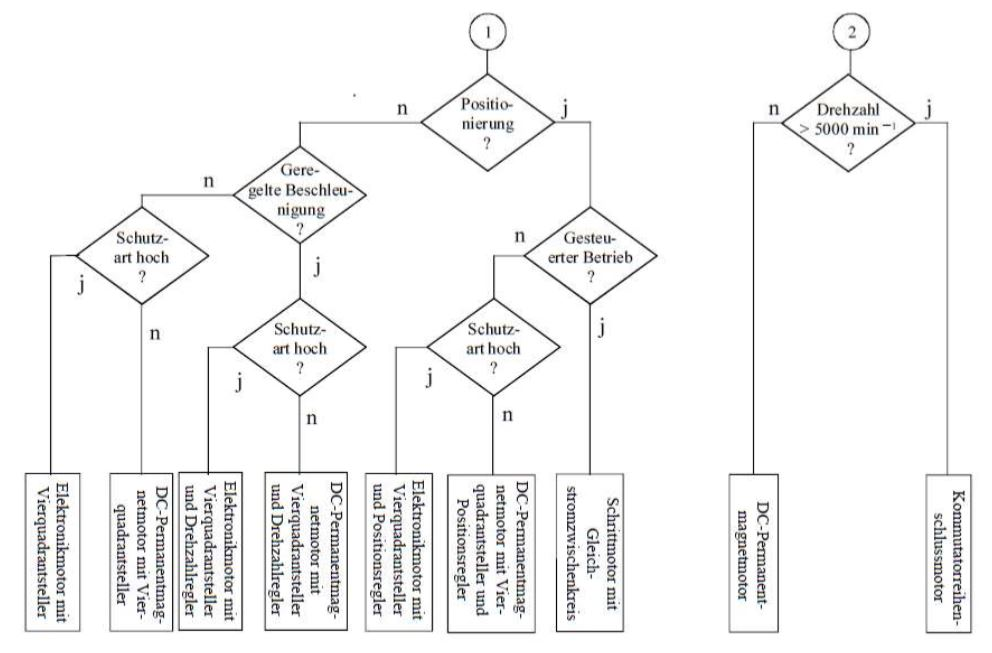
\includegraphics[scale=1]{images/Motorauswahl2}
\\
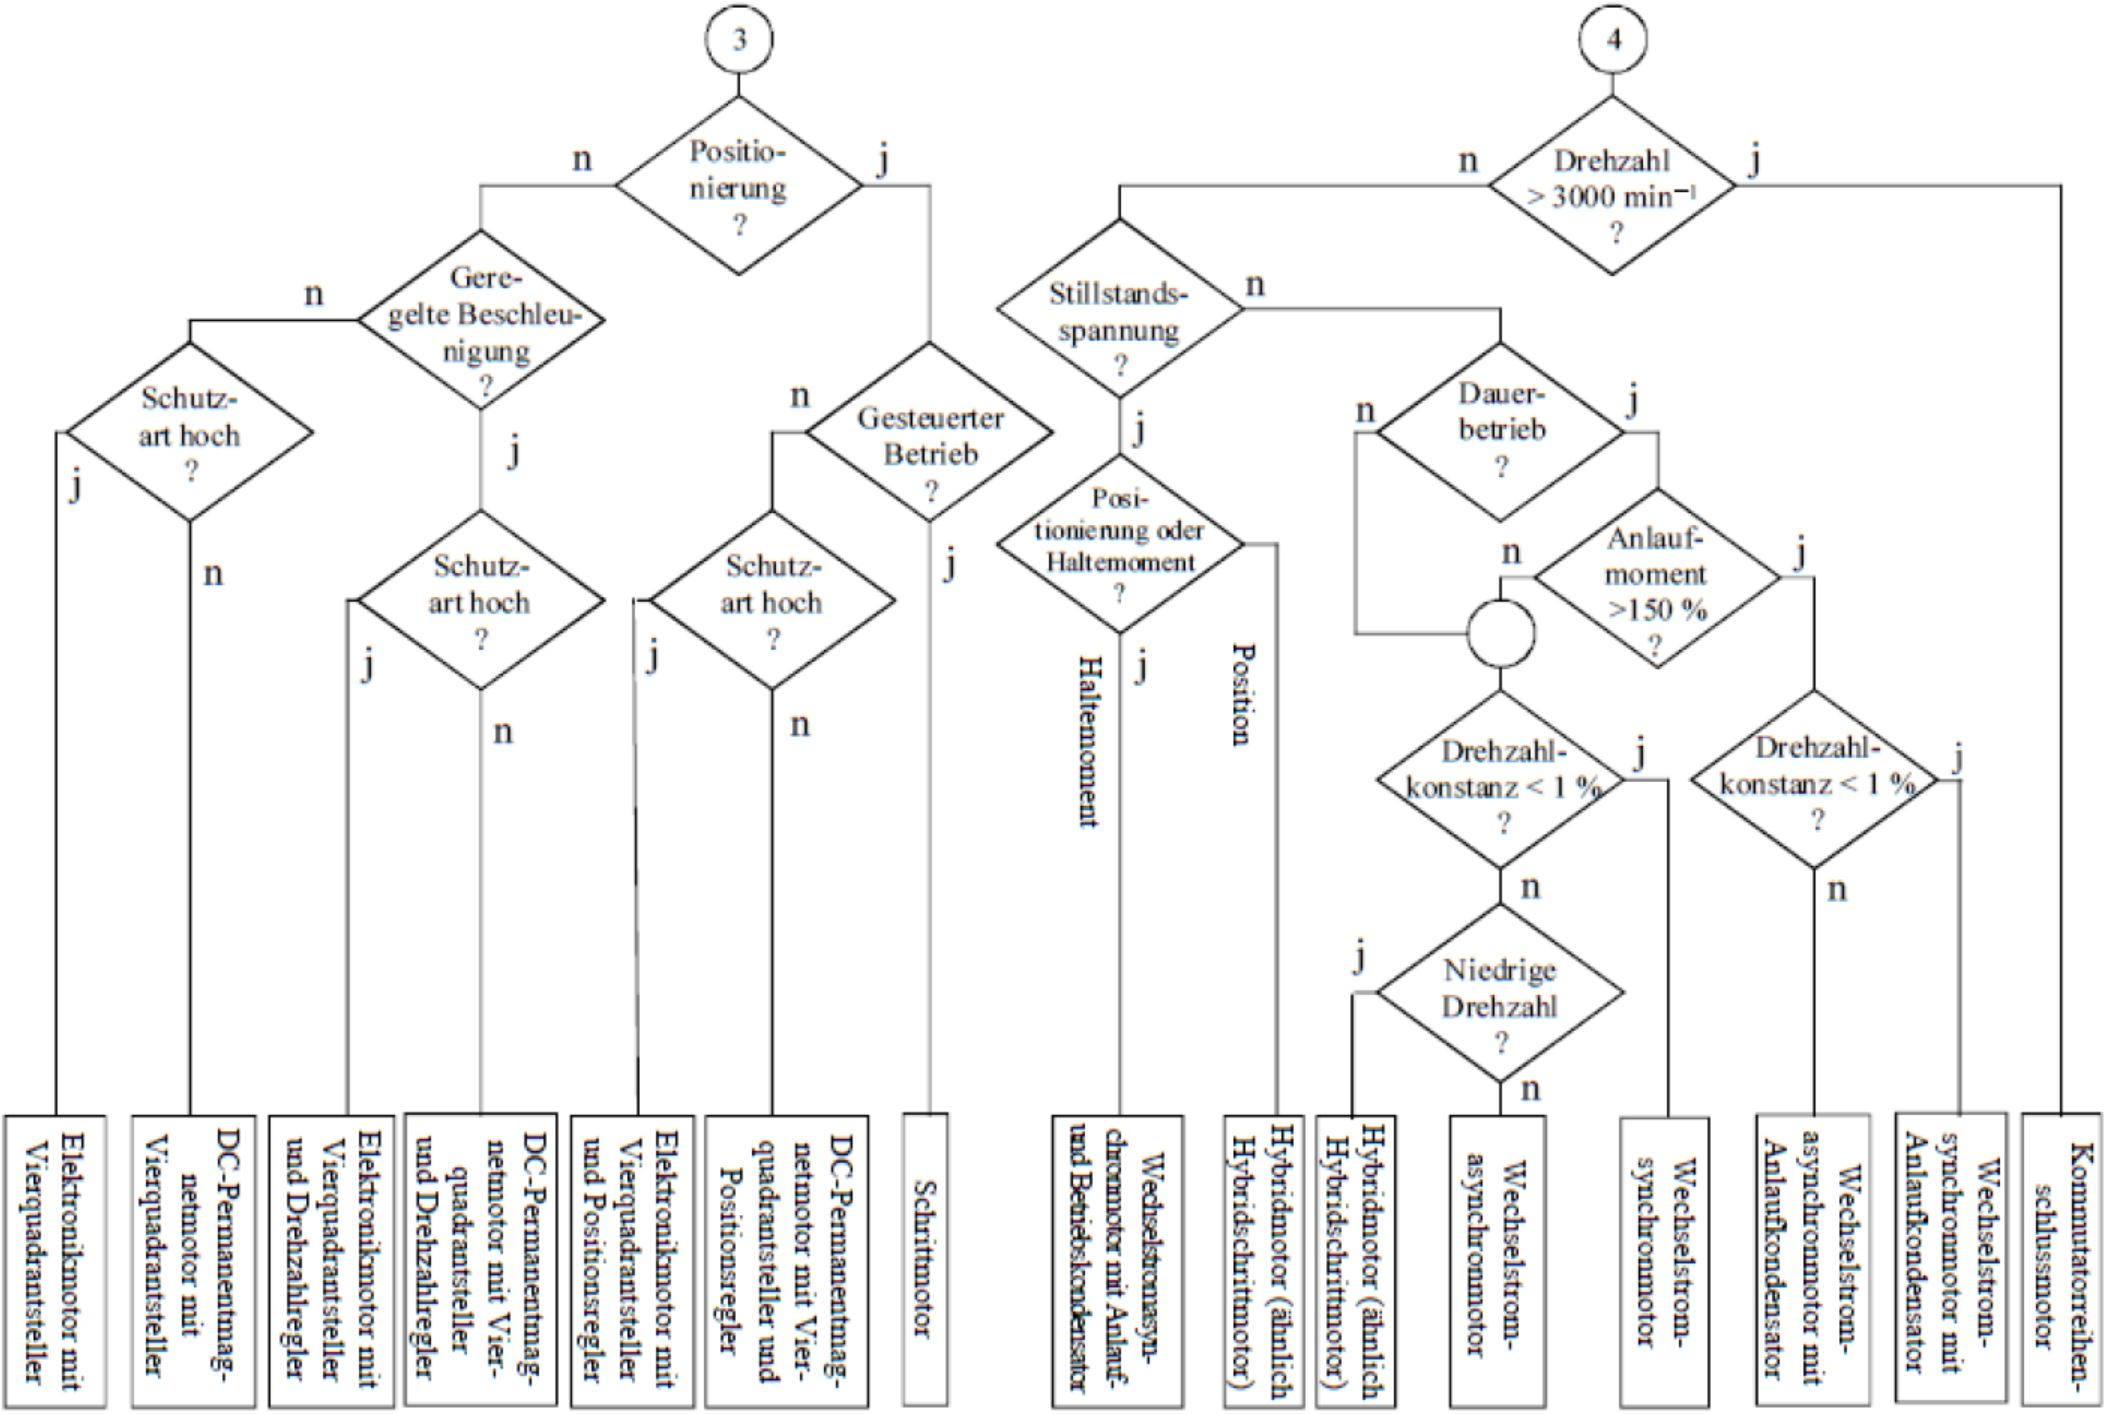
\includegraphics[scale=1]{images/Motorauswahl3}
\\
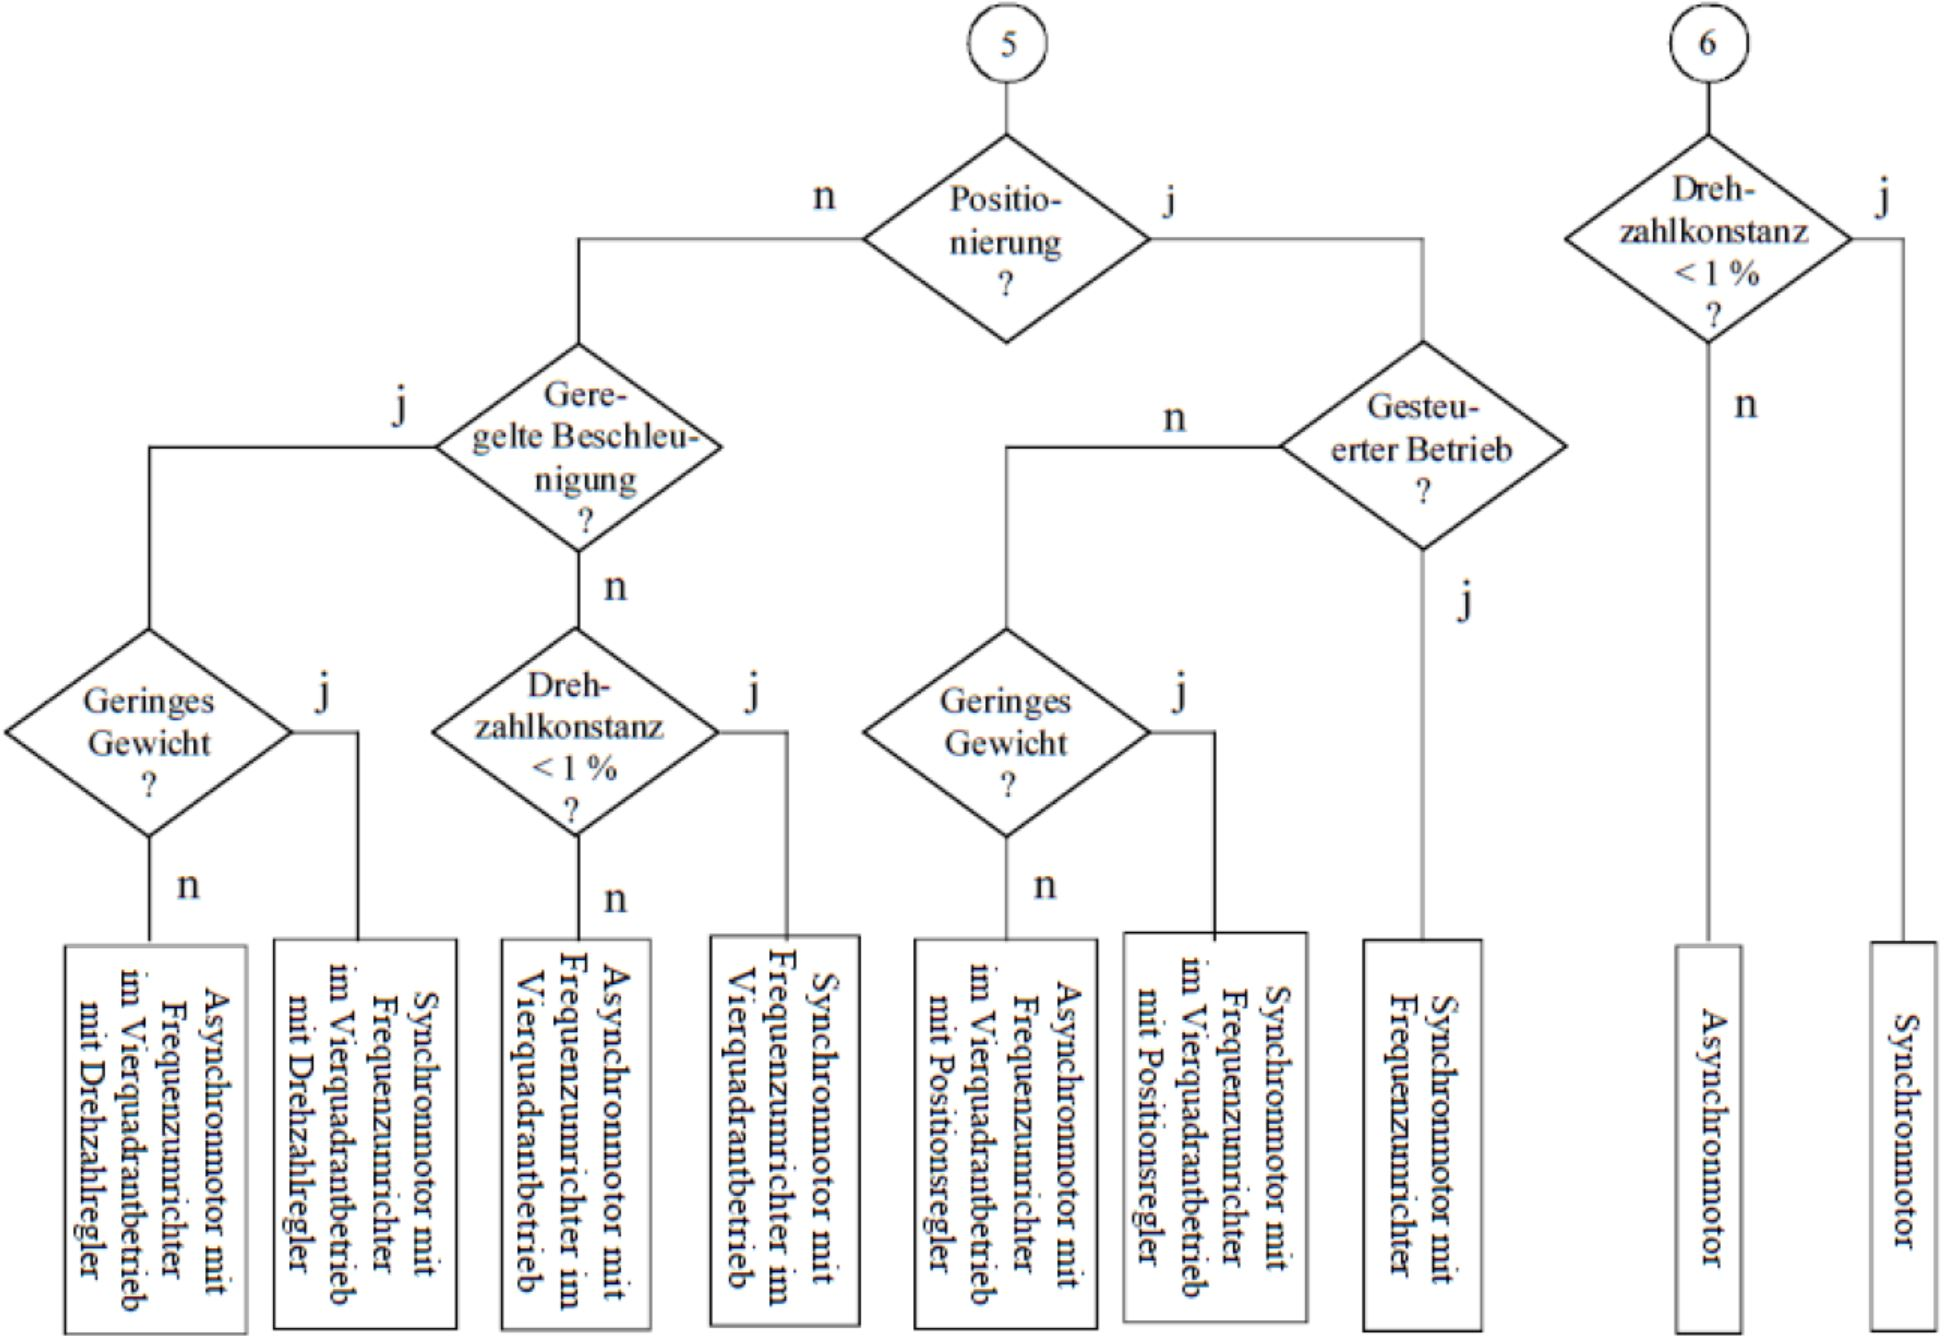
\includegraphics[scale=1]{images/Motorauswahl4}
\clearpage
\pagebreak
\addtocontents{toc}{\setcounter{tocdepth}{1}} %ToC ohnly shows section
%TODO Vektorprodukt/Kreuzprodukt
\section{Idiotenseite} 
%\subsection{Diverses}
\begin{tabbing}
	xxxxxxxxxxxxxxxxxxxxxxxxxxxx \= xxxxxxxxxxxxxxxxxxxxxxxxxxxxxx \= \kill
 	$f'(z) = \lim \limits_{\Delta z \rightarrow 0} \frac{f(z + \Delta z) -
	f(z)}{\Delta z}$ \> $(a + b)^n = \sum_{k=0}^{n} \binom n k a^{n-k} \cdot b^k$ \>
	$(a \pm b)^3 =a^3 \pm  3 a^{2} b + 3 a b^2 \pm b^3 $\\ \\
	$x_{1,2} = \dfrac{-b \pm \sqrt{b^2 - 4ac}}{2a}$ \> $\binom n k = \dfrac{n!}{k!
	\cdot (n-k)!}$ \> $(a \pm b)^4 =a^4 \pm  4 a^{3} b + 6a^2b^2 \pm 4 a b^3 +
	b^4$\\
\end{tabbing}
%\subsection{Reihenentwicklungen}
\begin{tabular}{llll}
\textbf{Geometrische Reihe}
	& $\sum\limits_{n=0}^{\infty} x^n$ 
	& $= \dfrac{1}{1-x}$
	& $|x| < 1$ \\
	
	& $\sum\limits_{k=0}^{\infty} k \, x^k$ & $= x \sum\limits_{k=1}^{\infty} k \,
	x^{k-1} = \dfrac{x}{(1-x)^2} $ 
	& $x \neq 1$ \\
    & $\sum\limits_{k=0}^{n} a_0\cdot q^k$ & $= a_0 \dfrac{1-q^{n+1}}{1-q}$
    & $q \neq 1$\\
\textbf{Binominalreihe} 
	& $\sum\limits_{n=0}^\infty \binom{\alpha}{n} x^n $ &$= (1+x)^\alpha$
	& $x \in (-1,1)$ \\
\textbf{E-Funktion}
	& $\sum\limits_{k = 0}^{\infty} \dfrac{x^k}{k!}$ &$ = e^x$
	& 
\end{tabular}

%\subsection{Kurven}
\begin{multicols}{4}
\subsubsection{e-Funktion}
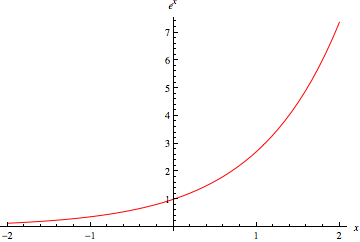
\includegraphics[width=4.5cm]{idiotenseite/images/Exp.png}
\subsubsection{Sinus-Funktion}
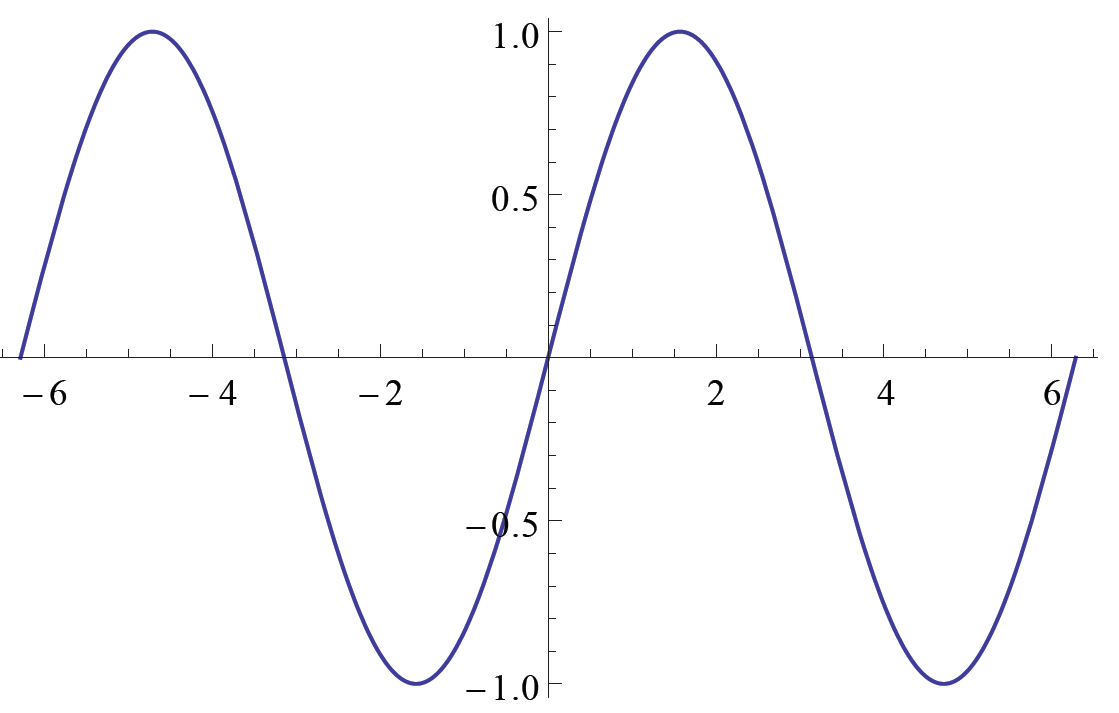
\includegraphics[width=4.5cm]{idiotenseite/images/sin.png}
\subsubsection{Cosinus-Funktion}
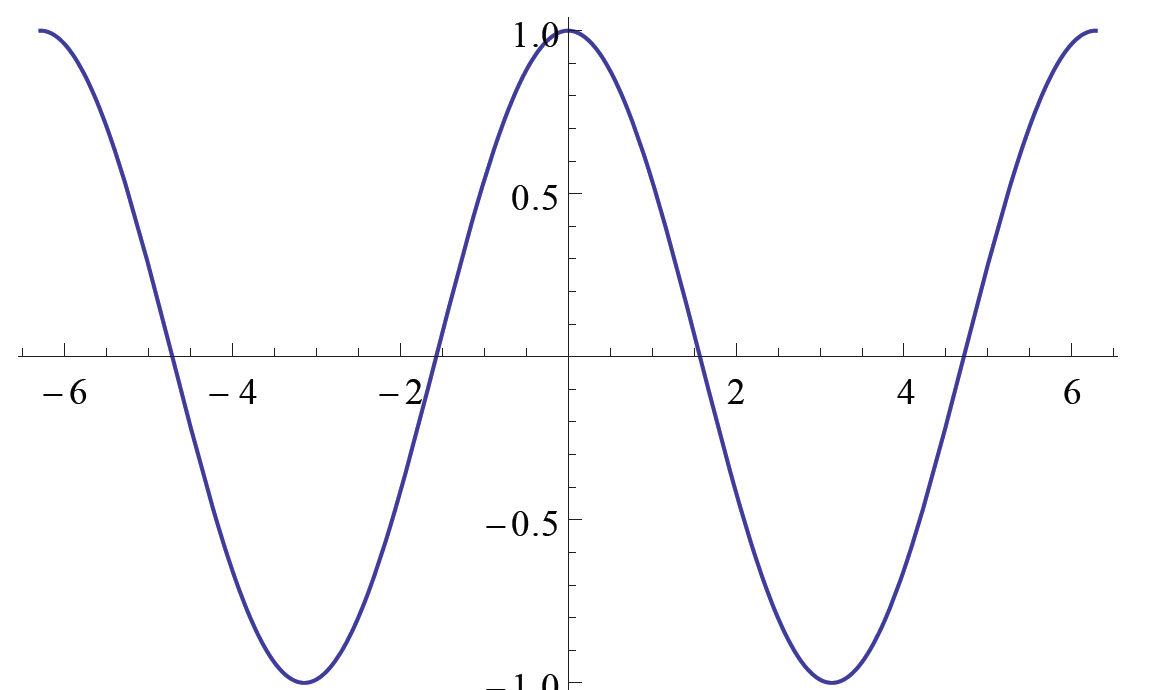
\includegraphics[width=4.5cm]{idiotenseite/images/cos.png}
\subsubsection{Tangens-Funktion}
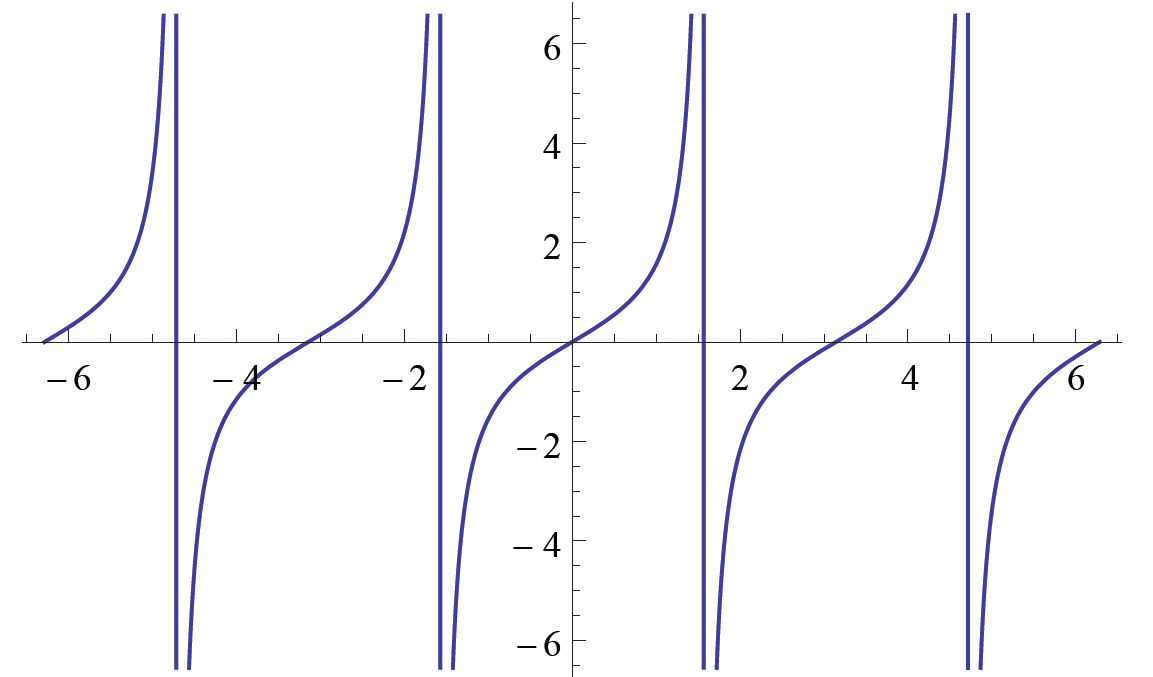
\includegraphics[width=4.5cm]{idiotenseite/images/tan.png}
\end{multicols}
%\subsection{Idiotenformel}
Wenn ihr wissen wollt was die Formel besagt dann kauft euch doch nächstes mal
die Pro Version der Formelsammlung. Arme Schmarotzer und asoziale Personen
dürfen gerne lange darüber Rätseln was das hier soll. Aber wer zu doof ist eine
Formelsammlung ehrlich zu erwerben hat sowieso keine Chance. Haha.\\
$\frac{1}{F_{Siedlungsfl\ddot ache}}\cdot\int\limits_{\vec{x} \in
Siedlungsfl\ddot ache} \frac{1}{\int\limits_{\vec{y}\in Siedlungsfl\ddot ache\ und \left|\vec{x}-\vec{y} \right|<BH}\vec{dy}} \int\limits_{\vec{y}\in Siedlungsfl\ddot ache\ und \left|\vec{x}-\vec{y} \right|<BH} \sqrt{\frac{2\cdot\left|\vec{x}-\vec{y}\right|}{1m}+1}-1\vec{dy}\vec{dx}\frac{DSE}{m^2}$

\newpage
\subsection{SI-Vorsätze}
\renewcommand{\arraystretch}{1.2}
\begin{tabularx}{\textwidth}{|X|X|X|X|X|X|l|}
	\hline
\textbf{Symbol}	&\textbf{Name}  &\textbf{Wert}  &\textbf{Binär}  &\textbf{Symbol}  &\textbf{Name}  &\textbf{Wert}
 \\ \hline 
da	& Deka    &$ 10^1 $   &    			     & d          & Dezi   &$ 10^{-1} $ 
\\ \hline
h	&Hekto    &$ 10^2 $   &                  & c          & Centi  &$ 10^{-2} $ 
\\ \hline
k	&Kilo     &$ 10^3 $   &$ 2^{10}=1024  $  & m          & Mili   &$ 10^{-3} $ 
\\ \hline
M	& Mega    &$ 10^6 $   &$ 2^{20} $        &$ y, \mu $  & Mikro  &$ 10^{-6} $
\\ \hline
G   &Giga     &$ 10^9 $   &$ 2^{30} $        & n          & Nano   &$ 10^{-9} $ 
\\ \hline
T	& Tera    &$ 10^{12} $&$ 2^{40} $        & p          & Piko   &$ 10^{-12} $
\\ \hline
P	&Peta	  &$ 10^{15} $&$ 2^{50} $	     & f          &	Femto  &$ 10^{-15} $
\\ \hline
\end{tabularx} 

%\subsection{GrichischesAlphabet}
\begin{multicols}{2}
	\subsubsection{klein}
	\begin{tabular}{ |l|l|l|l|l|l|l|l|}
		\hline
		$\alpha$&Alpha&$\theta$&Theta&o&o&$\tau$&Tau\\
		\hline
		$\beta$&Beta&$\vartheta$&Theta&$\pi$&Pi&$\upsilon$&Ypsilon\\
		\hline
		$\gamma$&Gamma&$\gamma$&Gamma&$\varpi$&Pi&$\phi$&Phi\\
		\hline
		$\delta$&Delta&$\kappa$&Kappa&$\rho$&Roh&$\varphi$&Phi\\
		\hline
		$\epsilon$&Epsilon&$\lambda$&Lambda&$\varrho$&Roh&$\chi$&Chi\\
		\hline
		$\varepsilon$&Epsilon&$\mu$&Mu&$\sigma$&Sigma&$\psi$&Psi\\
		\hline
		$\zeta$&Zeta&$\nu$&Nu&$\varsigma$&Sigma&$\omega$&Omega\\
		\hline
		$\eta$&Eta&$\xi$&Xi&&&&\\
		\hline
	\end{tabular}
	\columnbreak
	
	\subsubsection{gross}
	\begin{tabular}{|l|l|l|l|l|l|l|l|}
		\hline
		$\Gamma$&Gamma&$\Lambda$&Lambda&$\Sigma$&Sigma&$\Psi$&Psi\\
		\hline
		$\Delta$&Delta&$\Xi$&Xi&$\Upsilon$&Ypsilon&$\Omega$&Omega\\
		\hline
		$\Theta$&Theta&$\Pi$&Pi&$\Phi$&Phi&&\\
		\hline
	\end{tabular}
\end{multicols}
%\begin{sidewaystable}
\subsection{Einige unbestimmte Integrale\formelbuch{1074}}
\label{unbestimmte_integrale}
\begin{tabular}{|p{12cm}|p{12cm}|}
  \hline
  
    $ \int dx=x+C $ &
     $ \int{x^\alpha}dx=\frac{x^{\alpha+1}}{\alpha+1}+C,\ x \epsilon \mathbb
    R ^+,\ \alpha \epsilon \mathbb R \backslash \{ -1 \} $ \\\hline
     $ \int{\frac{1}{x}}dx=\ln \left| x \right| + C,\ x\neq0 $ &
     $ \int{e^x}dx=e^x+C $ \\\hline
     $ \int{a^x}dx=\frac{a^x}{\ln{a}}+C,\ a \epsilon \mathbb 
    R^+\backslash\{1\} $ &
     $ \int{ \sin{x}} dx = -\cos{x} + C $ \\\hline
     $ \int{\cos{x}} dx = \sin{x} + C $ &
     $ \int{\frac{dx}{\sin^2x}}=-\cot{x}+C,\ x\neq k\pi\ \mathrm{mit}\ k
    \epsilon \mathbb Z $ \\\hline
     $ \int{\frac{dx}{\cos^2x}}=\tan{x}+C,\ x\neq\frac{\pi}{2}+k\pi\
    \mathrm{mit} k \epsilon \mathbb Z $ & 
    
    %10. :
     $ \int{\sinh{x}}dx = \cosh{x}+C $ \\ \hline
     $ \int{\cosh{x}}dx = \sinh{x}+C $ &
     $ \int{\frac{dx}{\sinh^2x}}=-\coth{x}+C,\ x\neq0 $ \\\hline
     $ \int{\frac{dx}{\cosh^2x}}=\tanh{x}+C $ &
     $ \int{\frac{dx}{ax+b}} = \frac{1}{a}\ln \left|ax + b\right| + C,\
    a\neq 0,x\neq-\frac{b}{a} $ \\\hline
     $ \int{\frac{dx}{a^2x^2+b^2}}=\frac{1}{ab}\arctan{\frac{a}{b}x}+C,\
    a\neq0,\ b\neq0 $ &
     $
    \int{\frac{dx}{a^2x^2-b^2}}=\frac{1}{2ab}\ln{\left|\frac{ax-b}{ax+b}\right|}+C,\
    a\neq0,\ b\neq0,\ x\neq\frac{b}{a},\ x\neq-\frac{b}{a} $ \\\hline
     $
    \int{\sqrt{a^2x^2+b^2}}dx=\frac{x}{2}\sqrt{a^2x^2+b^2}+\frac{b^2}{2a}\ln{(ax+\sqrt{a^2x^2+b^2})}+C,\
    a\neq0,\ b\neq0 $ &
     $
    \int{\sqrt{a^2x^2-b^2}}dx=\frac{x}{2}\sqrt{a^2x^2-b^2}-\frac{b^2}{2a}\ln\left|ax+\sqrt{a^2x^2-b^2}\right|+C,\
    a\neq0,\ b\neq0,a^2x^2\geqq b^2$ \\\hline
     $
    \int\sqrt{b^2-a^2x^2}dx=\frac{x}{2}\sqrt{b^2-a^2x^2}+\frac{b^2}{2a}\arcsin\frac{a}{b}x+C,\
    a\neq0,\ b\neq0,\ a^2x^2\leqq b^2 $ &
    %20.:
     $
    \int\frac{dx}{\sqrt{a^2x^2-b^2}}=\frac{1}{a}\ln(ax+\sqrt{a^2x^2+b^2})+C,\
    a\neq0,\ b\neq0 $ \\\hline
     $
    \int\frac{dx}{\sqrt{a^2x^2-b^2}}=\frac{1}{a}\ln\left|ax+\sqrt{a^2x^2-b^2}\right|+C,\
    a\neq0,\ b\neq0,\ a^2x^2>b^2 $ &
     $ \int\frac{dx}{\sqrt{b^2-a^2x^2}}=\frac{1}{a}\arcsin\frac{a}{b}x+C,\
    a\neq0,\ b\neq0,\ a^2x^2<b^2 $ \\\hline
     Die Integrale $\int\frac{dx}{X}, \int\sqrt{X}dx,
    \int\frac{dx}{\sqrt{X}}$ mit $X=ax^2+2bx+c,\ a\neq0 $ werden durch 
    die Umformung $X=a(x+\frac{b}{a})^2+(c-\frac{b^2}{a}) $ und die
    Substitution $ t=x+\frac{b}{a} $ in die oberen 4 Zeilen
    transformiert. & $ \int\frac{xdx}{X}=\frac{1}{2a}\ln\left|X\right|-\frac{b}{a}\int\frac{dx}{X},\
    a\neq0,\ X=ax^2+2bx+c $ \\\hline
     $ \int\sin^2axdx=\frac{x}{2}-\frac{1}{4a}\cdot\sin2ax+C,\ a\neq0 $ &
     $ \int\cos^2axdx=\frac{x}{2}+\frac{1}{4a}\cdot\sin2ax+C,\ a\neq0 $ \\\hline
     $ \int\sin^naxdx=-\frac{sin^{n-1}ax\cdot\cos
    ax}{na}+\frac{n-1}{n}\int\sin^{n-2}axdx,\ n \epsilon \mathbb N,\ a\neq0 $ &
     $ \int\cos^naxdx=\frac{\cos^{n-1}ax\cdot\sin
    ax}{na}+\frac{n-1}{n}\int\cos^{n-2}axdx,\ n\epsilon \mathbb N,\ a\neq0 $
    \\\hline
     $ \int\frac{dx}{\sin ax} =
    \frac{1}{a}\ln\left|\tan\frac{ax}{2}\right|+C,\ a\neq0,\ x\neq
    k\frac{\pi}{a}\ \mathrm{mit}\ k\epsilon\mathbb Z$ &
    %30.:
     $ \int\frac{dx}{\cos
    ax}=\frac{1}{a}\ln\left|\tan(\frac{ax}{2}+\frac{\pi}{4})\right|+C,\ a\neq0,\
    x\neq\frac{\pi}{2a}+k\frac{\pi}{a}\ \mathrm{mit}\ k\epsilon\mathbb Z $
    \\\hline
     $\int\tan axdx=-\frac{1}{a}\ln\left|\cos ax\right|+C,\ a\neq0,\
    x\neq\frac{\pi}{2a}+k\frac{\pi}{a} \mathrm{mit}\ k\epsilon\mathbb Z$ &
     $\int\cot axdx=\frac{1}{a}\ln\left|\sin ax\right|+C,\ a\neq0,\ x\neq
    k\frac{\pi}{a} \mathrm{mit} k\epsilon\mathbb Z $ \\ \hline
     $ \int x^n\sin axdx=-\frac{x^n}{a}\cos ax+\frac{n}{a}\int x^{n-1}\cos
    axdx,\ n\epsilon\mathbb N,\ a\neq0 $ &
    $ \int x^n\cos axdx=\frac{x^n}{a}\sin ax-\frac{n}{a}\int x^{n-1}\sin
    axdx,\ n\epsilon\mathbb N,\ a\neq0 $ \\ \hline
     $ \int x^ne^{ax}dx=\frac{1}{a}x^ne^{ax}-\frac{n}{a}\int
    x^{n-1}e^{ax}dx,\ n\epsilon\mathbb N,\ a\neq0 $ &
     $ \int e^{ax}\sin bxdx=\frac{e^{ax}}{a^2+b^2}(a\sin bx-b\cos bx)+C,\
    a\neq0,\ b\neq0 $  \\ \hline
     $ \int e^{ax}\cos bxdx=\frac{e^{ax}}{a^2+b^2}(a\cos bx + b\sin bx)+C,\
    a\neq0,\ b\neq0 $ &
     $ \int\ln x dx = x(\ln x-1)+C,\ x\epsilon\mathbb R^+ $ \\ \hline
     $ \int x^\alpha \cdot \ln xdx =
    \frac{x^{\alpha+1}}{(\alpha+1)^2}\lbrack(\alpha+1)\ln x-1\rbrack + C,\
    x\epsilon\mathbb R^+,\ \alpha\epsilon\mathbb R\backslash\{-1\} $ & \\ \hline
    %FF1 Seite 496
    
\end{tabular}
\end{sidewaystable}
%%\begin{sidewaystable}
\subsection{Ableitungen elementarer Funktionen\formelbuch{436}}
\label{unbestimmte_integrale}
\renewcommand{\arraystretchOriginal}{2.5}
\begin{tabular}{|l|l||l|l|}
  \hline
  \textbf{Funktion} & \textbf{Ableitung} & \textbf{Funktion} &
  \textbf{Ableitung}\\\hline
  $C$ (Konstante) & 0 & $\sec x$ & $\dfrac{\sin x}{\cos^2 x}$ \\
  $x$ & 1 & $\sec^{-1} x$ & $\dfrac{-\cos x}{\sin^2 x}$\\
  $x^n$ ($n\in\mathbb{R}$) & $nx^{n-1}$ & $\arcsin x \quad (|x| < 1)$ &
  $\dfrac{1}{\sqrt{1-x^2}}$\\
  $\dfrac{1}{x}$ & $-\dfrac{1}{x^2}$ & $\arccos x \quad (|x| < 1)$ &
  $-\dfrac{1}{\sqrt{1-x^2}}$\\
  $\dfrac{1}{x^n}$ & $-\dfrac{n}{x^{n+1}}$ & $\arctan x$ & $\dfrac{1}{1+x^2}$\\
  $\sqrt{x}$ & $\dfrac{1}{2\sqrt{x}}$ & arccot $x$ & $-\dfrac{1}{1+x^2}$\\
  $\sqrt[n]{x}\quad (n\in\mathbb{R}, n \neq 0, x > 0)$ &
  $\dfrac{1}{n\sqrt[n]{x^{n-1}}}$ & arcsec $x$ & $\dfrac{1}{x\sqrt{x^2-1}}$\\
  $\mathrm{e}^x$ & $\mathrm{e}^x$ & arcossec $x$ & $-\dfrac{1}{x\sqrt{x^2-1}}$\\
  $\mathrm{e}^{bx}\quad (b\in\mathbb{R})$ & $b\mathrm{e}^{bx}$ & $\sinh x$ &
  $\cosh x$\\
  $a^x\quad (a > 0)$ & $a^x\ln a$ & $\cosh x$ & $\sinh x$\\
  $a^{bx}\quad (b\in\mathbb{R}, a > 0)$ & $ba^{bx}\ln a$ & $\tanh x$ &
  $\dfrac{1}{\cosh^2 x}$\\
  $\ln x$ & $\dfrac{1}{x}$ & $\coth x \quad(x \neq 0)$ & $-\dfrac{1}{\sinh^2 x}$\\
  $\log_a{x} \quad (a > 0, a \neq 1, x > 0)$ &
  $\dfrac{1}{x}\log_a{\mathrm{e}}=\dfrac{1}{x\ln a}$ & Arsinh $x$ &
  $\dfrac{1}{\sqrt{1+x^2}}$\\
  $\lg x \quad (x > 0)$ & $\dfrac{1}{x}\lg \mathrm{e}\approx \dfrac{0.4343}{x}$
  & Arcosh $x \quad (x > 1)$ & $\dfrac{1}{\sqrt{x^2-1}}$\\
  $\sin x$ & $\cos x$ & Artanh $x \quad (|x| < 1)$ & $\dfrac{1}{1-x^2}$\\
  $\cos x$ & $-\sin x$ & Arcoth $x \quad (|x| > 1)$ & $-\dfrac{1}{x^2-1}$\\
  $\tan x \quad (x\neq(2k+1)\dfrac{\pi}{2}, k\in\mathbb{Z})$ & $\dfrac{1}{\cos^2
  x}=\sec^2 x$ & $[f(x)]^n \quad (n\in\mathbb{R})$ & $n[f(x)]^{n-1}f'(x)$\\
  $\cot x \quad (x\neq k\pi, k\in\mathbb{Z})$ & $\dfrac{-1}{\sin^2 x}=-cosec^2x$ & $\ln f(x) \quad (f(x)> 0)$ & $\dfrac{f'(x)}{f(x)}$\\
  \hline
\end{tabular}
\renewcommand{\arraystretchOriginal}{1.5}
%\end{sidewaystable}

\subsection{Dreiecksformeln}
\begin{tabular}{lll}
	& \parbox{9.5cm}{
		\textbf{Cosinussatz} \\
		$$c^2 = a^2 + b^2 - 2 \cdot a \cdot b \cdot \cos \gamma$$\\
		\textbf{Sinussatz} \\
		$$\frac{a}{\sin \alpha} = \frac{b}{\sin \beta} = \frac{c}{\sin \gamma} = 2r =
		\frac{u}{\pi}$$
		\textbf{Pythagoras beim Sinus}\\
		$$\sin^2(b)+\cos^2(b)=1 \qquad \tan(b)=\frac{\sin(b)}{\cos(b)}$$}
		
	& \parbox{8cm}{
		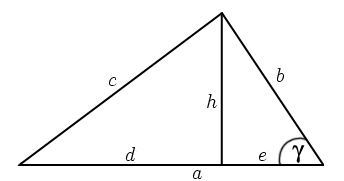
\includegraphics[width=6cm]{./idiotenseite/images/cosinussatz.png}}
\end{tabular}
\begin{center}
	\begin{multicols}{2}
		$\sin \beta = \frac ba =\frac{\text{Gegenkathete}}{\text{Hypotenuse}}$\\
		$\cos \beta = \frac ca =\frac{\text{Ankathete}}{\text{Hypotenuse}}$\\
		$\tan \beta = \frac cb =\frac{\text{Gegenkathete}}{\text{Ankathete}}$\\
		$\cot \beta = \frac cb =\frac{\text{Ankathete}}{\text{Gegenkathete}}$\\
	\end{multicols}
\end{center}

	
\subsection{Funktionswerte für Winkelargumente}
	\begin{multicols}{4}	
	\begin{tabular}[c]{|p{0.5cm}|p{0.4cm}||p{0.5cm}|p{0.5cm}|p{0.5cm}|}
	    	\hline
			deg & rad & sin & cos & tan\\
			\hline
			0\symbol{23} & 0 & 0 & 1 & 0\\
			\hline
			30\symbol{23} & $\frac{\pi}{6}$ & $\frac{1}{2}$ & $\frac{\sqrt{3}}{2}$ &
			$\frac{\sqrt{3}}{3}$\\
			\hline
			45\symbol{23} & $\frac{\pi}{4}$ & $\frac{\sqrt{2}}{2}$ & $\frac{\sqrt{2}}{2}$
			& 1\\
			\hline
			60\symbol{23} & $\frac{\pi}{3}$ & $\frac{\sqrt{3}}{2}$ & $\frac{1}{2}$ &
			$\sqrt{3}$\\
			\hline			
	\end{tabular} \\
	
	\begin{tabular}[c]{|p{0.7cm}|p{0.7cm}||p{0.7cm}|p{0.7cm}|}
	    	\hline
			deg & rad & sin & cos\\
			\hline
			90\symbol{23} & $\frac{\pi}{2}$ & 1 & 0\\
			\hline	
			120\symbol{23} & $\frac{2\pi}{3}$ & $\frac{\sqrt{3}}{2}$ & $-\frac{1}{2}$ \\
			\hline
			135\symbol{23} & $\frac{3\pi}{4}$ & $\frac{\sqrt{2}}{2}$ & $-\frac{\sqrt{2}}{2}$\\
			\hline
			150\symbol{23} & $\frac{5\pi}{6}$ & $\frac{1}{2}$ & $-\frac{\sqrt{3}}{2}$\\
			\hline
	\end{tabular} \\
	
	\begin{tabular}[c]{|p{0.7cm}|p{0.7cm}||p{0.7cm}|p{0.7cm}|}
	  	\hline
		deg & rad & sin & cos\\
		\hline
		180\symbol{23} & $\pi$ & 0 & -1\\
		\hline	
		210\symbol{23} & $\frac{7\pi}{6}$ & $-\frac{1}{2}$ & $-\frac{\sqrt{3}}{2}$\\
		\hline
		225\symbol{23} & $\frac{5\pi}{4}$ & $-\frac{\sqrt{2}}{2}$ & $-\frac{\sqrt{2}}{2}$\\
		\hline
		240\symbol{23} & $\frac{4\pi}{3}$ & $-\frac{\sqrt{3}}{2}$ & $-\frac{1}{2}$\\
		\hline
	\end{tabular} \\
	
	\begin{tabular}[c]{|p{0.7cm}|p{0.7cm}||p{0.7cm}|p{0.7cm}|}
    	\hline
		deg & rad & sin & cos\\
		\hline
		270\symbol{23} & $\frac{3\pi}{2}$ & -1 & 0\\
		\hline	
		300\symbol{23} & $\frac{5\pi}{3}$ & $-\frac{\sqrt{3}}{2}$ & $\frac{1}{2}$\\
		\hline
		315\symbol{23} & $\frac{7\pi}{4}$ & $-\frac{\sqrt{2}}{2}$ & $\frac{\sqrt{2}}{2}$\\
		\hline
		330\symbol{23} & $\frac{11\pi}{6}$ & $-\frac{1}{2}$ & $\frac{\sqrt{3}}{2}$\\
		\hline
	\end{tabular}					
\end{multicols}

\begin{minipage}{13cm}
	\subsection{Periodizität}
	$\cos(a+k\cdot2\pi)=\cos(a) \qquad \sin(a+k\cdot2\pi)=\sin(a) \qquad
	(k \in \mathbb{Z})$
	\subsection{Quadrantenbeziehungen}
	\begin{tabbing}
    	xxxxxxxxxxxxxxxxxxxxxxxxxxxxxxxxxx \= \kill
	  	$\sin(-a)=-\sin(a)$ \> $\cos(-a)=\cos(a)$\\
		$\sin(\pi - a)=\sin(a)$ \> $\cos(\pi - a)=-\cos(a)$\\
		$\sin(\pi + a)=-\sin(a)$ \> $\cos(\pi +a)=-\cos(a)$\\
		$\sin\left(\frac{\pi}{2}-a \right)=\sin\left(\frac{\pi}{2}+a \right)=\cos(a)$ \>
		$\cos\left(\frac{\pi}{2}-a \right)=-\cos\left(\frac{\pi}{2}+a \right)=\sin(a)$  
    \end{tabbing}
\end{minipage}
\begin{minipage}{5cm}
	

\subsection{Ableitungen}

\begin{tikzpicture}
	[	inner sep = 2mm,
		sin/.style={rectangle,minimum width=1.2cm,minimum height=1cm,rounded corners=5pt,draw=black,top color=green!20!black!50},
		abl/.style={rectangle}
	]
	\node at (1.2,0) (sin1) [sin] {$\sin$};
	\node at (0,-1.2) (cos2) [sin] {$-\cos$};
	\node at (1.2,-2.4) (sin2) [sin] {$-\sin$};
	\node at (2.4,-1.2) (cos1) [sin] {$\cos$};
	
	\draw[thick,black,->] (sin1.east) .. controls +(right:0.6cm) and +(up:0.6cm) ..  (cos1.north)
	node [pos=0.5,above](abl) {$\frac{d}{dx}$};
	\draw[thick,black,->] (cos1.south) .. controls +(down:0.6cm) and +(right:0.6cm) .. (sin2.east)
	node [pos=0.5,below](abl) {$\frac{d}{dx}$};
	\draw[thick,black,->] (sin2.west) .. controls +(left:0.6cm) and +(down:0.6cm) .. (cos2.south)
	node [pos=0.5,below](abl) {$\frac{d}{dx}$};
	\draw[thick,black,->] (cos2.north) .. controls +(up:0.6cm) and +(left:0.6cm) .. (sin1.west)
	node [pos=0.5,above](abl) {$\frac{d}{dx}$};
\end{tikzpicture}
\end{minipage}
\begin{multicols}{2}
	\subsection{Additionstheoreme}
	$\sin(a \pm b)=\sin(a) \cdot \cos(b) \pm \cos(a) \cdot \sin(b)$\\
	$\cos(a \pm b)=\cos(a) \cdot \cos(b) \mp \sin(a) \cdot \sin(b)$\\	
	$\tan(a \pm b)=\dfrac{\tan(a) \pm \tan(b)}{1 \mp \tan(a) \cdot \tan(b)}$
	\columnbreak
	
	\subsection{Doppel- und Halbwinkel}	
	$\sin(2a)=2\sin(a)\cos(a)$\\
	$\cos(2a)=\cos^2(a)-\sin^2(a)=2\cos^2(a)-1=1-2\sin^2(a)$\\
	$\cos^2 \left(\frac{a}{2}\right)=\frac{1+\cos(a)}{2} \qquad
	\sin^2 \left(\dfrac{a}{2}\right)=\frac{1-\cos(a)}{2}$
\end{multicols}
%\begin{multicols}{2}
	%%\subsection{Produkte}
		$\sin(a)\sin(b)=\frac{1}{2}(\cos(a-b)-\cos(a+b))$\\
		$\cos(a)\cos(b)=\frac{1}{2}(\cos(a-b)+\cos(a+b))$\\
		$\sin(a)\cos(b)=\frac{1}{2}(\sin(a-b)+\sin(a+b))$\\
	%\subsection{Euler-Formeln} 

	$\sin(x) = \frac{1}{2j} \left(e^{jx} - e^{-jx}\right) \qquad
	\cos(x) = \frac{1}{2} \left(e^{jx} + e^{-jx}\right)$ \\
	$e^{x+jy} = e^x \cdot e^{jy} = e^x \cdot \left(\cos(y) + j\sin(y)\right)$ \\
	$e^{j\pi} = e^{-j\pi} = -1$ \\
%	\columnbreak
	
%	\subsection{Summe und Differenz}
		$\sin(a)+\sin(b)=2 \cdot \sin \left(\frac{a+b}{2}\right) \cdot
		\cos\left(\frac{a-b}{2}\right)$\\
		$\sin(a)-\sin(b)=2 \cdot \sin \left(\frac{a-b}{2}\right) \cdot
		\cos\left(\frac{a+b}{2}\right)$\\
		$\cos(a)+\cos(b)=2 \cdot \cos \left(\frac{a+b}{2}\right) \cdot
		\cos\left(\frac{a-b}{2}\right)$\\
		$\cos(a)-\cos(b)=-2 \cdot \sin \left(\frac{a+b}{2}\right) \cdot
		\sin\left(\frac{a-b}{2}\right)$\\
		$\tan(a) \pm \tan(b)=\dfrac{\sin(a \pm b)}{\cos(a)\cos(b)}$\\
%\end{multicols}

\subsection{Geradengleichung Interpolieren}
$ y(x)=y_0 + \frac{y_1 - y_0}{x_1 - x_0}(x-x_0) $
\clearpage
\subsection{Quellenumwandlung}
\begin{tabular}{cccp{6cm}}
Lineare Stromquelle		& $\Longleftrightarrow$ & Lineare Spannungsquelle & Formeln \\
\raisebox{-.8\totalheight}{\includegraphics[width=2.8cm]{idiotenseite/images/ersatz_strom.jpg}}&
&
\raisebox{-.8\totalheight}{\includegraphics[width=2.8cm]{idiotenseite/images/ersatz_spannung.jpg}}
&
$I_q = \frac{U_q}{R_i} = U_q \cdot G_{i Spannungsquelle}$ \newline
$U_q = \frac{I_q}{G_i} = I_q \cdot R_{i Stromquelle}$ \newline
Der Wiederstand/Leitwert bleibt gleich \newline \\
\end{tabular}
\subsection{Superposition}
\textbf{Vorgehen:}
\begin{multicols}{2}
\begin{enumerate}
  \item Alle Quellen bis auf eine entfernen
  \item Restliche Quellen ersetzen: Stromquelle $\rightarrow$ Unterbruch,
  Spannungsquelle $\rightarrow$ Kurzschluss
  \item Teilströme mit der verbleibenden Quelle berechnen
  \item Für alle anderen Quellen das vorgehen wiederholen
  \item Alle Teilströme/-spannungen zusammenzählen
\end{enumerate}
\end{multicols}
\subsection{Einschaltvorgänge}
\subsubsection{Kondensator}
\input{idiotenseite/elektrotechnik/subsections/einschalt_kondensator}
\subsubsection{Spule}
\input{idiotenseite/elektrotechnik/subsections/einschalt_spule}


\subsection{ohmsche Leistung}
\begin{multicols}{3}
	$P=U \cdot I = I^2 \cdot R = \frac{U^2}{R}$ \\
	$P= I^2 \cdot \omega L = \frac{U^2}{\omega L}$\\
	$P= I^2 \cdot \omega C = \frac{U^2}{\omega C}$
\end{multicols}
\subsection{Strom- Spannungsquellen-Verschiebung}
\input{idiotenseite/tikz/elektrotechnik/UQuellenverschiebung1.tex}
\input{idiotenseite/tikz/elektrotechnik/UQuellenverschiebung2.tex}
\input{idiotenseite/tikz/elektrotechnik/IQuellenverschiebung1.tex}
\input{idiotenseite/tikz/elektrotechnik/IQuellenverschiebung2.tex}      
\subsection{Allgemein zeitabhängige Grössen}
	\begin{tabular}{|ll|ll|}
    \hline
	\multicolumn{2}{|l}{Arithmetischer Mittelwert, Gleichwert, Linearer MW} 
	    	& \multicolumn{2}{l|}{$X_0 = \overline{X} = X_m = \frac {1} {T} \int\limits_{t_0}^{t_0+T}
	    	x(t)dt$} \\
	\hline
	Quadratischer MW, Leistung 
		& $X^2 = \frac {1} {T} \int\limits_{t_0}^{t_0+T} x^2(t)dt$ 
		& MW $n$. Ordnung
		& $X^n = \frac {1} {T} \int\limits_{t_0}^{t_0+T} x^n(t)dt$ \\
	\hline
	Effektivwert (RMS) 
		& $X = \sqrt{X^2} = \sqrt{\frac{1}{T} \int\limits ^{t_0+T}_{t_0}{x^2(t)dt}}$
		& Gleichrichtwert 
		& $X_{|m|} = \bar{|X|} = \frac{1}{T} \int\limits_{t_0}^{t_0+T}{|x(t)| dt}$ \\
	\hline
\end{tabular}
\begin{sidewaystable}
\subsection{Eigenschaften unterschiedlicher Schwingungsformen}
\begin{center}
\begin{tabular}{|l|c|c|c|c|c|c|c|c|}
\hline
	Schwingungsform & Funktion & Gleichrichtwert & Formfaktor &
	Effektivwert & Scheitelfaktor & \textbf{$X_0$} & \textbf{$X^2$} & \textbf{var(X)} \\
\hline
	Formel &
	&
	$\overline{\left|x\right|} = \frac1T\int_{0}^{T}\left| x(t)\right|dt$&
	$\frac{X}{\overline{\left|x\right|}}$&
	$X = \sqrt{X^2} = \sqrt{\frac{1}{T} \int\limits ^{t_0+T}_{t_0}{x^2(t)dt}}$&
	$k_{s}=\frac{X_{\mathrm{max}}}{X_{\mathrm{eff}}}$&
	&
	&
	\\
\hline
	\includegraphics[width=2cm]{idiotenseite/images/table_sine_wave.png} &
	$A\cdot\sin(t)$ &
	$\frac{2}{\pi} \approx 0.637$ &
	$\frac{\pi}{2\sqrt{2}} \approx 1.11$ &
	$\frac{1}{\sqrt{2}}\approx 0.707$ &
	$\sqrt{2}\approx 1.414$ &
	$0$ &
	$\frac{A^2}{2}$ &
	$\frac{A^2}{2}$ \\
\hline	
	\includegraphics[width=2cm]{idiotenseite/images/table_full-wave_rectified_sine.png} &
	$A\cdot|\sin(t)|$ &
	$\frac{2}{\pi} \approx 0.637$ &
	$\frac{\pi}{2\sqrt{2}} \approx 1.11$ &
	$\frac{1}{\sqrt{2}} \approx 0.707$ &
	$\sqrt{2} \approx 1.414$  &
	$\frac{2A}{\pi}$ & $\frac{A^2}{2}$ & $\frac{A^2}{2}-\frac{4A^2}{\pi^2}$
	\\
\hline
	\includegraphics[width=2cm]{idiotenseite/images/table_half-wave_rectified_sine.png} &
	$\begin{cases} A\cdot\sin (t) & 0<t<\pi  \\ 0 & \text{True}\end{cases}$ &
	$\frac{1}{\pi}\approx 0.318$ &
	$\frac{\pi}{2}\approx 1.571$ &
	$\frac{1}{2} = 0.5$	&
	2  &
	$\frac{A}{\pi}$ &
	$\frac{A^2}{4}$ & $\frac{A^2}{4}-\frac{A^2}{\pi^2}$
	\\
\hline
	\includegraphics[width=2cm]{idiotenseite/images/table_triangle_wave.png} &
	$A\cdot\Lambda(t)$ &
	$\frac{1}{2}= 0.5$ &
	$\frac{2}{\sqrt{3}}\approx 1.155$ &
	$\frac{1}{\sqrt{3}}
	\approx 0.557$ &
	$\sqrt{3} \approx 1.732$ &
	$0$ &
	$\frac{A^2}{3}$ &
	$\frac{A^2}{3}$ \\
\hline	
	\includegraphics[width=2cm]{idiotenseite/images/table_square_wave.png} &
	$\begin{cases} A & 0<x<t \\ 0 & \text{True}\end{cases}$ &
	$1$ &
	$1$ &
	$1$ &
	$1$ &
	$0$ &
	$A^2$ &
	$A^2$ \\
\hline	
	DC&
	1&
	$1$ &
	$1$ &
	$1$ &
	$1$  &
	-&
	-&
	-\\
\hline	
	\includegraphics[width=2cm]{idiotenseite/images/table_pulse_wide_wave.png} &
	&
	$\frac{t_1}{T}$ & $\sqrt{\frac{T}{t_1}}$ & $\sqrt{\frac{t_1}{T}}$ & $\sqrt{\frac{T}{t_1}}$ &
	$A\frac{t}{T}$ &
	$A^2\frac{t}{T}$ &
	$\frac{A^2t}{T}-\frac{A^2t^2}{T^2}$\\
\hline
\end{tabular}
\end{center}
\end{sidewaystable}



\section{TODO}
  	\subsection{Grundelemente}
  	\begin{tabular}{p{1.5cm} p{4.3cm} |p{1.5cm} p{4.3cm}| p{1.5cm} p{4.3cm}}
  		\multicolumn{2}{l}{\textbf{Ohmscher Widerstand R}}
  		& \multicolumn{2}{l}{\textbf{Kapazitität C}}
  		& \multicolumn{2}{l}{\textbf{Induktivität L}} \\
  		\multicolumn{2}{l}{$u$ und $i$ können sprunghaft ändern}
  		& \multicolumn{2}{l}{$\mathbf{u}$ \textbf{kann nicht sprunghaft ändern}}
  		& \multicolumn{2}{l}{$\mathbf{i}$ \textbf{kann nicht sprunghaft ändern}} \\
  		
  		\multirow{2}{1.5cm}{
  			\includegraphics[width=1.5cm]{./images/zeigerdiag-r.png}}
  		& $u(t) = R \cdot i(t)$ 
  		& \multirow{2}{1.5cm}{\includegraphics[width=1.5cm]{./images/zeigerdiag-c.png}}
  		& $u(t) = \frac{1}{C} \int\limits_0^t i(\tau) d\tau + u(0)$
  		& 
  		\multirow{2}{1.5cm}{\includegraphics[width=1.5cm]{./images/zeigerdiag-l.png}}
  		&$u(t) = L \frac{di(t)}{dt}$\\
  		
  		&$i(t) = \frac{u(t)}{R}$
  		& & $i(t) = C \frac{d u(t)}{dt}$
  		& & $i(t) = \frac{1}{L} \int\limits_0^t u(\tau) d\tau + i(0)$\\
  		
  		& $\underline{Z}_R = R$
  		& & $\underline{Z}_C = \frac{1}{j \omega C} = - \frac{j}{\omega C}$
  		& & $\underline{Z_L} = j \omega L$\\
  		
  		\parbox{1.7cm}{\small{nicht linear:}}
  		& $R_=(u) = \frac{U}{I(u)}, r_D = \frac{\diff U}{\diff I}\lvert_{U_0}$
  		& & $X_C = -\frac{1}{\omega C} \quad B_C = \omega C$
  		& & $X_L = \omega L
  		\quad B_L = -\frac{1}{\omega L}$ \\
  		
  		& $P=I^2 \cdot R = \frac{U^2}{R}$
  		& & $Q_C= - U^2 \cdot \omega C = - \frac{I^2}{\omega C}$
  		& & $Q_L= I^2 \cdot \omega L = \frac{U^2}{\omega L}$\\
  		
  		& & & $W_C=\frac12 C U_C^2$
  		& &$W_L=\frac12 L I_L^2$
  	\end{tabular}

\subsection{Begriffe der Impedanz und Admitanz}
\begin{tabular}{lllll}
	Scheinwiderstand & & $Z = \frac{U_{eff}}{I_{eff}} $ & $ =
	\sqrt{R^2+X^2}$ & Ohm\\ Komplexer Widerstand & Impedanz & $\underline Z = R + jX = Z \cdot e^{j \varphi}$ 
	& $  = \dfrac{\underline{U}}{\underline{I}} = \dfrac{\underline{U}\cdot\underline{U}^{\ast}}{\underline{S}^*} =  = \dfrac{U^2}{\underline{S}^*} = 
	\dfrac{\underline{S}}{I^2}$ & Ohm\\
	Komplexer Leitwert & Admittanz & $\underline Y = G + jB =
	\frac{1}{\underline Z} = \frac{1}{Z}e^{-j\varphi}$ & $= \frac{\underline{I}}{\underline{U}}$ &  Siemens\\
	Wirkwiderstand & Resistanz & $R = \Real(\underline Z) $ & $ = Z
	\cdot cos(\varphi)$ & Ohm\\
	Wirkleitwert & Konduktanz & $G = \Real(\underline Y) $ & $ \neq \frac{1}{R}$ &
	Siemens\\
	Blindwiderstand & Reaktanz & $X = \Imag(\underline Z) $ & $ = Z
	\cdot sin(\varphi)$ & Ohm\\
	Blindleitwert & Suszeptanz & $B = \Imag( \underline Y) $ & $ \neq \frac{1}{X}$
	& Siemens\\
	Phasenverschiebung & & $\varphi = \varphi_u - \varphi_i =
	\arctan\left(\frac{\Imag(\underline{Z})}{\Real(\underline{Z})}\right)$ & &
	Radiant\\
	
\end{tabular}
	
\subsection{Formeln Übung 5}
\begin{tabular}[b]{|C{4cm}| P{8cm} | P{5cm}|}
    \hline
    \textbf{Polradwinkel}&
    \[ p(\delta)=\frac{U_p \cdot U_1}{X_d} sin(\delta) \]&
    $ \delta$ = Polradwinkel \newline
    $ U_p = $ Polradspannung \newline
    $ L_d =$ Synchroninduktivität (?)
    \\ \hline
    
    \textbf{Polpaarzahl}&
    $ p=\frac{60 \cdot f}{n} $&
    $ \left[n= \frac{1}{min}\right] $
    \\ \hline
    
    &
    \[  \frac{sin(\delta)}{2\pi f L_d}=\frac{sin(\delta ')}{2\pi f L_d '} \] &
    \\ \hline       
\end{tabular}
\clearpage
\pagebreak

\end{document}
